\documentclass[12pt,a4paper]{scrartcl}
\usepackage[utf8]{inputenc}
\usepackage[T1]{fontenc}
\usepackage{ngerman}
\usepackage{placeins}
%\usepackage[ngerman]{babel}  % use babel for multi-ling or english
%
%\usepackage{amsmath,amssymb,amstext}

\usepackage{amsmath}
\usepackage{wrapfig}
\usepackage{multirow}
%\usepackage{sv}
\usepackage{pgf}
\usepackage{pst-sigsys}
\usepackage{multido}
\usepackage{pdfpages}
\usepackage{listings}
\usepackage{color}
\definecolor{light-gray}{gray}{0.95}


% fuer Zitate
\usepackage[numbers]{natbib}
\usepackage{nomencl,longtable} 
% Festlegung Art der Zitierung - Havardmethode: Abkuerzung Autor + Jahr
%\bibliographystyle{alphadin}

\bibliographystyle{unsrt}
%\usepackage[twoside=false,
%            left=2cm,
%            right=2cm,
%            top=2cm,
%            bottom=3cm]{geometry}
\usepackage{tikz}
\usepackage{siunitx}

\usetikzlibrary{shapes,arrows,automata,backgrounds,calendar}
\usepackage[europeancurrents,
						europeanvoltages,
						europeanresistors,
						cuteinductors,
						europeanports]{circuitikz}
\usepgflibrary{plotmarks}
\usepackage{trfsigns}
\usepackage{pstricks} \SpecialCoor
\makeatletter
\def\psStartPunkt(#1){\pst@getcoor{#1}\pst@tempA 
  \pstVerb{\pst@tempA 
           \pst@number\psyunit div /cp.Y exch def 
           \pst@number\psxunit div /cp.X exch def }}
\def\psVektor{\pst@object{psVektor}}
\def\psVektor@i(#1){%
  \pst@killglue%
  \pst@getcoor{#1}\pst@tempA%
  \begin@SpecialObj%
  \rput(! cp.X cp.Y ){\psline[arrowsize=6pt]{->}(0,0)(#1)%
    \psarc[arrows=->,arrowsize=4pt](0,0){1}{0}{!\pst@tempA exch atan}%
    \psline[linestyle=dotted](1.5,0)}%
  \end@SpecialObj%
  \pstVerb{tx@Dict begin \pst@tempA \pst@number\psyunit div 
            cp.Y add /cp.Y exch def 
            \pst@number\psxunit div 
            cp.X add /cp.X exch def end}  
  \ignorespaces%
}

\usepackage{nicefrac}
\usepackage{float}
\usepackage[bottom=3cm, top=2cm, left=2.5cm, right=2cm]{geometry}

%%%%%%%%%%%%%%%%%%%%%%%%%%%%%%%%%%%%%%%%%%%%%%%%%%%%%%%%%%%%%%%%%%%%%%%%%%%%%%%%
%%% Headings
%%%
%\usepackage[automark]{scrpage2}
%\pagestyle{scrheadings}
%\ihead[]{}
%\chead[]{}
%\ohead[]{}
%\ifoot[]{}
%\cfoot[]{}
%\ofoot[]{}

%%%%%%%%%%%%%%%%%%%%%%%%%%%%%%%%%%%%%%%%%%%%%%%%%%%%%%%%%%%%%%%%%%%%%%%%%%%%%%%%
%%% Commands
%%%
\renewcommand{\vec}[1]{\boldsymbol{#1}}
\newcommand{\mat}[1]{\boldsymbol{#1}}
\renewcommand{\lstlistingname}{Listing}

\DeclareMathAlphabet{\mathpzc}{OT1}{pzc}{m}{it}
\newcommand{\z}{\mathpzc{z}}

\newcommand{\nomunit}[1]{% 
\renewcommand{\nomentryend}{\hspace{2em}\hspace*{\fill}#1}}
\newcommand{\parDiff}[2]{\frac{\partial #1}{\partial #2}}
\newcommand{\coord}[2]{\left(#1, #2 \right)}
%%%%%%%%%%%%%%%%%%%%%%%%%%%%%%%%%%%%%%%%%%%%%%%%%%%%%%%%%%%%%%%%%%%%%%


%\title{Übung Drehfeldmaschinen \\mit Umrichter}

\author{}

%\date{Graz, am \today{}}

\parindent0pt

%%%%%%%%%%%%%%%%%%%%%%%%%%%%%% Main %%%%%%%%%%%%%%%%%%%%%%%%%%%%%%%%%% 


\begin{document}
\begin{titlepage}
\pagestyle{empty} \enlargethispage*{25cm}\samepage{

\vspace*{-1.5cm}
\begin{center}
\begin{minipage}[!h]{18cm}
\hspace*{-1.1cm}

\includegraphics[width=3.3cm]{igte}
\begin{tabular}{p{10cm}}
\centering{
\Large Institut für Grundlagen und Theorie\\
der Elektrotechnik\\[2mm]
Technische Universität Graz
}
\end{tabular}

\includegraphics[width=3.3cm]{TUG}
\end{minipage}

%\vspace*{2.4cm}
\vspace*{5cm}
%
\Huge {Seminararbeit:\\
Finite Elemente Software \\zur Lösung von \\Elektrostatik- und stationären Strömungsfeld-Problemen} %
\vspace*{2cm}

\Large{vorgelegt von:\\
Tobias Florian Lafer (01530012)\\
am 21.08.2019} 
\vspace{8cm}


\Large{Betreuer: Dipl-Ing. Paul Baumgartner, BSc BSc}\vspace*{2cm}\vfill

\end{center}}%
\clearpage 

\tableofcontents
\newpage

\end{titlepage}
%



\newcommand{\screenshot}[3]{
\begin{figure}[ht]
 \centering
\hspace*{-.05\textwidth}
\makebox[\textwidth]{
  \includegraphics[width = 19cm]{#3}}
 \caption{#1} \label{fig:#2} 
\end{figure}
\FloatBarrier
}


\newcommand{\screenshotWidth}[4]{
\begin{figure}[ht]
 \centering
\hspace*{-.05\textwidth}
\makebox[\textwidth]{
  \includegraphics[width = {#4 cm}]{#3}}
 \caption{#1.} \label{fig:#2} 
\end{figure}
\FloatBarrier
}

\newcommand{\screenshotHeight}[4]{
\begin{figure}[ht]
 \centering
\hspace*{-.05\textwidth}
\makebox[\textwidth]{
  \includegraphics[height = {#4 cm}]{#3}}
 \caption{#1} \label{fig:#2} 
\end{figure}
\FloatBarrier
}

\newcommand{\doubleScreenShot}[9]{

  \begin{figure}[!ht]
	  \caption*{#9}
    \begin{minipage}{0.49\linewidth}\centering
      %\rule{\linewidth}{0.5\linewidth}  % Platzhalter
			\includegraphics[width={#4}\textwidth]{#3} 
      \caption{#1.}\label{fig:#2}
    \end{minipage}
    \hfill
    \begin{minipage}{0.49\linewidth}\centering
      %\rule{\linewidth}{0.5\linewidth}  % Platzhalter
			\includegraphics[width={#8}\textwidth]{#7}
      \caption{#5}\label{fig:#6}
    \end{minipage}
		
  \end{figure} 
\FloatBarrier
}




\section*{Zusammenfassung}

\section*{Zusammenfassung}
\vspace*{2cm}
\begin{large}

Die Methode der finiten Elemente ist eine der bekanntesten und am weitesten Verbreiteten Methoden zur Lösung von Randwertproblemen in unterschiedlichsten Disziplinen. Das Institut für Grundlagen und Theorie der Elektrotechnik hat zu diesem Zwecke vor vielen Jahren mit der Entwicklung einer kommerziell Verwendbaren Software für eben jene Probleme auf dem Bereich der Elektrotechnik entwickelt. Aus diesen Bemühungen sind die Softwarepakete EleFAnT3D und EleFAnt2D entstanden.\newline

Beim Einsatz in der Lehre geht der Fokus einer solchen Software jedoch weg von hoher Optimierung und großem Funktionsumfang hin zu einfacher Bedienung und leichter Erweiterbarkeit des Source-Codes. Aus diesen Überlegungen heraus wurde die Entwicklung einer, auf der Open-Source-Software Gmsh und dem weit verbreiteten Mathematik-Programm Matlab\textregistered, basierenden Software zur Lösung oben genannter Probleme zum Einsatz speziell in der Lehre gestartet.\newline

Diese Seminararbeit versteht sich als ein Teil vergangener, laufender und noch folgender Seminararbeiten zur sukzessiven Entwicklung dieser Software.  \newline
Ziel dieser Seminararbeit ist die Implementierung der Lösung von zweidimensionalen, ebenen elektrostatischen und stationären Strömungsfeld-Problemen, sowie die automatisierte Generierung des Gitters mittels der Software Gmsh, dessen Import und Verarbeitung in der Software.

\end{large}


\section{Theorie}
\subsection{Die Methode der finiten Elemente}
\label{sec:fem_theory}
Die nachfolgenden Abschnitte in diesem Kapitel basieren, bis auf Abschnitt \ref{sec:finite_elements_and_shape_functions}, im wesentlichen auf \cite{SMS_VO_skript}.\newline

Die analytische Lösung eines Randwertproblems, wie jenes definiert in (\ref{eq:operatorgleichung}), ist nur in sehr wenigen Fällen möglich. Zur numerischen Lösung existieren daher verschiedenste Methoden, wobei eine der Prominentesten die \textit{Methode der finiten Elemente} darstellt. Bei dieser Methode wird das zu untersuchende Problemgebiet $\Omega$ in viele einzelne Teilgebiete unterteilt, in welchen jeweils die gesuchte Funktion $u(x)$ durch Verwendung von Ansatzfunktionen (zum Beispiel Polynomen) approximiert wird. \newline

Ein Beispiel für ein Randwertproblem ist
\begin{equation}
L\{u(x)\} - f(x) = 0
\label{eq:operatorgleichung}
\end{equation}
mit $u = \overline{u} \ \forall x\in \Gamma_D$ als dirichletschen, und $\parDiff{u}{n}(x) = u_N \ \forall x \in \Gamma_N $ als neumannschen Randbedingungen, $L$ als Differentialoperator, $f$ als gegebener und $u$ als gesuchter Funktion.\newline

Als häufige Ansätze für die numerische Berechnung dienen dabei das sogenannte \textit{Ritzsche Verfahren} (Spezialfall einer Variationsmethode) oder das \textit{Galerkinsche Verfahren} (Spezialfall einer Residuenmethode). Diese Verfahren führen auf ein lineares Gleichungssystem (\ref{eq:gleichungssystem}) mit den Werten der gesuchten Funktion $u$ an den Elementknoten als Unbekannte $\vec{u_{ges}}$.

\begin{equation}
\vec{A} \cdot \vec{u_{ges}} = \vec{r}
\label{eq:gleichungssystem}
\end{equation}

Die Elemente der Matrix $\vec{A}$ und des Rechtsseitenvektors $\vec{r}$ ergeben sich aus den  (i.A. differentiellen) Zusammenhängen im Problemgebiet, den vorgegebenen Randwerten und der Geometrie sowie deren Unterteilung.\newline

\subsection{Das Ritzsche Verfahren}
Physikalische Systeme gehorchen in vielen Fällen sogenannten \textit{Extremalprinzipien}. Ein solches Prinzip bezeichnet die Eigenschaft eines Systems einen Zustand einzunehmen in dem eine bestimmte Größe minimal oder maximal ist. Zum Beispiel verläuft die Bewegung eines dynamischen Systems immer so dass dessen Bewegungsenergie minimal ist. Eine bekannte Anwendung dieses Prinzips ist der \textit{Lagrange Foralismus}\newline

Ein in der Elektrotechnik vorkommendes Extremalprinzip ist das \textit{Kelvinsche Prinzip} welches besagt dass sich die Ladungsverteilung in einem elektrostatischen System so einstellt, dass die Energie in diesem System minimal ist.\newline
Mathematisch ausgedrückt muss somit die elektrostatische Energie 
\begin{equation}
\label{eq:functional}
W(V) = \frac{1}{2} \int\displaylimits_{\Omega} \vec{E}\cdot\vec{D} d\Omega = \frac{\epsilon_0}{2} \int\displaylimits_{\Omega} \left(-\mathit{grad}V\right)^2 d\Omega
\end{equation}
 mit $\vec{E} = -\mathit{grad}(V)$ und $\vec{D} = \epsilon_0 \vec{E}$, minimiert werden. Wählt man nun eine Potentialfunktion $V^* = V + \beta \eta$, wobei $V$ den wahren Potentialverlauf, $\eta$ einer \textbf{beliebigen} Abweichung von $V^*$ gegenüber dem wahren Verlauf, und $\beta$ einem numerischen \textit{Schaarparameter} entspricht, so kann über 
 \begin{equation}
 \label{eq:first_variation}
 \frac{dW(V^*)}{d\beta}\bigg\vert_{\beta = 0} \beta = \frac{d}{d\beta} \left(\frac{\epsilon_0}{2} \int\displaylimits_{\Omega} \left(- \mathit{grad}(V + \beta \eta)\right)^2 d\Omega \right)\bigg\vert_{\beta = 0} \beta \overset{!}{=} 0
 \end{equation} 
 der wahre Verlauf $V$ bestimmt werden.\newline
 Die aus ($\ref{eq:first_variation}$) resultierenden Differentialgleichungen bezeichnet man als \textit{Euler-Lagrange Differentialgleichungen}. Die Idee des Ritzschen Verfahrens ist nun, einen Ansatz für $V^*$ zur Lösung der Differentialgleichungen zu wählen. \newline
 Wählt man als Ansatz für $V*$
 \begin{equation}
 V* = \phi_0 + \sum_{k = 1}^{N} c_k \phi_k
 \end{equation}
 so können nach Einsetzen in (\ref{eq:first_variation}) die $c_j$ über ein lineares Gleichungssystem ermittelt werden. $\phi_0$ und $\phi_k$ bezeichnet man als \textit{Testfunktionen}.\newline
 
 Man bezeichnet (\ref{eq:functional}) als \textit{Funktional} und (\ref{eq:first_variation}) als \textit{erste Variation} des Funktionals.\newline
 Hat man nun, wie bei einem Randwertproblem üblich, eine Differentialgleichung gegeben, so muss zuerst ein äquivalentes Funktional gefunden werden. Für einige Fälle ist dies über Tabellenbücher möglich.


\subsection{Das Galerkinsche Verfahren}
Die Operatorgleichung aus (\ref{eq:operatorgleichung}) ist für alle Werte von $u(x)$ exakt erfüllt. Wählt man nun für $u$ einen Approximationsansatz $u^*$, so ist (\ref{eq:operatorgleichung}) nun im Allgemeinen nicht mehr exakt erfüllt. Man definiert $\epsilon := L\{ u^* \} -f$ als das sogenannte \textit{Residuum} (Rest) und möchte die Parameter der Approximationsfunktion so verändern dass 
\begin{equation}
\label{eq:weighted_residuum}
\int\displaylimits_{\Omega}\epsilon w d\Omega = \int\displaylimits_{\Omega} (L\{ u^* \} -f)w d\Omega= 0
\end{equation}
ist. $w$ bezeichnet hierbei eine \textbf{beliebige} Gewichtsfunktion. Man spricht nun von der \textit{Methode der gewichteten Residuen}.\newline


Wählt man nun als Ansatz für $u*$
\begin{equation}
u* = \phi_0 + \sum_{k = 1}^{N} c_k \phi_k
\end{equation}

und für die Gewichtsfunktion $w$
\begin{equation}
	w = \phi_0 + \sum_{k = 1}^{N} \alpha_k\phi_k
\end{equation}

mit $\alpha_k \neq 0$ so spricht man von der \textit{Galerkin-Bubnov-Metode} oder vom \textit{Galerkinschen Verfahren}. Durch Einsetzen der Ansätze für $u^*$ und $w$ in (\ref{eq:weighted_residuum}) lassen sich die $c_k$ über ein lineares Gleichungssystem bestimmen. Die $\alpha_k$ müssen nicht berechnet werden, da sie als beliebig und $\neq 0$ angenommen werden. 


\subsection{Finite Elemente und Formfunktionen}
\label{sec:finite_elements_and_shape_functions}
Ein häufiger Ansatz zur Unterteilung des Problemgebietes ist jener der Unterteilung in Dreiecke bzw. Tetraeder. Innerhalb jedes dieser Elemente wird die gesuchte Funktion $u$ aus \ref{eq:operatorgleichung}, im Weiteren auch Potential genannt, durch einfache Funktionen, meist Polynome erster oder zweiter Ordnung, angenähert.\newline
Für ein Element, welches durch $N$ Knoten definiert wird lautet ein möglicher Ansatz 
\begin{equation}
\label{eq:ansatz_potential}
u(x,y) = \sum_{k = 1}^{N_e}N_k^e u_k
\end{equation}
wobei die Funktionen $N_k^e$ als \textit{Formfunktionen} des $e$-ten Elements bezeichnet werden. Sie besitzen im $k$-ten Elementknotenknoten den Wert $1$ und in allen Anderen den Wert $0$. \newline
Für ein Dreieck mit einem Knoten an jeder Ecke ($N = 3$) ergeben sich lineare Funktionen für $N_k^e$, für Dreiecke mit zusätzlichen Knoten in der Mitte jeder Seite ($N=6$) quadratische Funktionen usw. \newline
Da die Funktionen für $N_k^e$ nur von der Geometrie des jeweiligen Elements abhängen bleiben einzig die $u_k$ als gesuchte Parameter, welche durch Verwendung des Ansatzes aus ($\ref{eq:ansatz_potential}$) im z.B. Galerkinschen Verfahren ermittelt werden können.\newline

Wie aus ($\ref{eq:ansatz_potential}$) erkennbar, müssen für jedes Element die $N_k^e$ separat ermittelt werden da sie von der jeweiligen Elementgeometrie abhängen. Betrachtet man nun jedes finite Element in einem lokalen Koordinatensystem, welches im Weiteren durch die Variablen $\xi,\eta$ dargestellt wird, und verwendet die Formfunktionen auch zur Beschreibung der Elementgeometrie, so spricht man von \textit{isoparametrischen finiten Elementen.}\newline
Die Formfunktionen müssen dabei nur einmalig für einen bestimmten Typ von finten Elementen (z.B. lineare Dreicke) einmalig ermittelt werden. Die Zusammenhänge für Geometrie und Potential lauten dann wie folgt:
\begin{equation}
\label{ref:ansatz_isoparam}
u = \sum_{k = 1}^{N} N_k(\xi, \eta) u_k \quad x = \sum_{k = 1}^{N} N_k(\xi, \eta) x_k  \quad y = \sum_{k = 1}^{N} N_k(\xi, \eta) y_k \nonumber
\end{equation}
wobei $x_k$ und $y_k$ die Koordinaten des $k$-ten Knoten darstellen. Sinnvollerweise sind die jeweiligen finiten Elemente im lokalen $\xi,\eta$-Koordinatensystem geradlinig angesetzt. (Siehe Abbildung \ref{fig:quadratic_element} ) Die Krümmung und Verzerrung im globalen Koordinatensystem ergibt sich anschließend durch (\ref{ref:ansatz_isoparam}).



\subsubsection{Lineare Dreieckselemente}
\label{sec:linear_triangles}
Das isoparametrische lineare Finite Dreieckselement ist im lokalen $\xi,\eta$-Koordinatensystem wie in Abbildung \ref{fig:linear_element} gezeigt dargestellt. \newline

\begin{wrapfigure}{r}{8cm}
	\begin{center}
		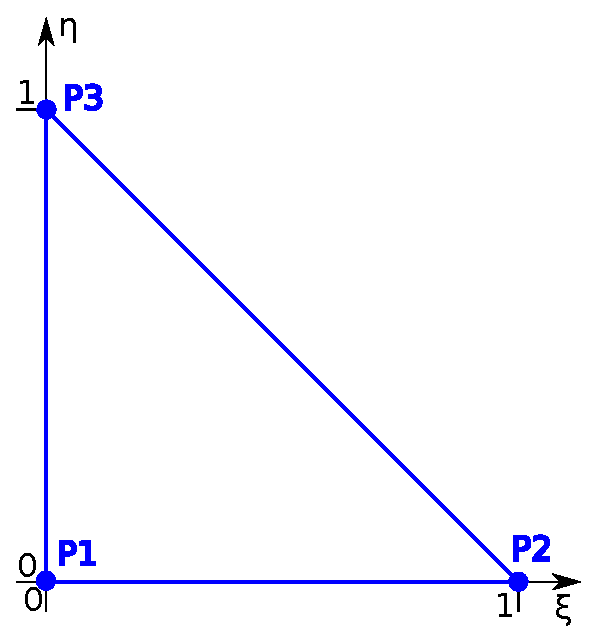
\includegraphics[scale=0.65]{pics/linear_element.eps}
	\end{center}
	\caption{Ansatz für lineares Element}
	\label{fig:linear_element}
\end{wrapfigure}

Die Koordinaten der drei Elementknoten lauten wie folgt:
\begin{align}
&P_1 = \coord{0}{0}, \quad P_2 = \coord{0}{1} \\
&P_3 = \coord{1}{0} \nonumber
\end{align}

Als Ansatz für die Potentialfunktion bzw. die globalen Koordinaten $x$ und $y$ wählt man folgenden Ansatz:
\begin{equation}
 \label{eq:linear_triangle_eq}
u(\xi, \eta) = c_0 + c_1 \xi + c_2 \eta
\end{equation}
Die drei Unbekannten $c_0$, $c_1$ und $c_2$ können durch Einsetzen der Koordinaten der Elementknoten ermittelt werden. 
\begin{align}
P_1:&\ u(0,0) = u_1 = c_0\\
P_2:&\ u(1,0) = u_2 = c_0 + c_1 \nonumber \\
P_3:&\ u(0,1) = u_3 = c_0 + c_2 \nonumber
\end{align}
 bzw. unter Verwendung der Matrixschreibweise:
 \begin{equation}
 \label{eq:linear_triangle_matrix_eq}
 \underbrace{
 \begin{bmatrix}
 1 & 0 & 0 \\
 1 & 1 & 0 \\
 1 & 0 & 1
 \end{bmatrix}}_{\mat{A}} \cdot 
\underbrace{
 \begin{Bmatrix}
 c_0 \\ c_1 \\ c_2
 \end{Bmatrix}}_{\vec{c}} = 
\underbrace{
 \begin{Bmatrix}
 u_1 \\ u_2 \\ u_3
 \end{Bmatrix}}_{\vec{u}}
 \end{equation}
 
 Die Lösung $\vec{c} = \mat{A}^{-1}\cdot\vec{u}$ lautet:
 \begin{equation}
\begin{Bmatrix}
c_0 \\ c_1 \\ c_2
\end{Bmatrix} = 
\begin{bmatrix}
1 & 0 & 0 \\
-1 & 1 & 0 \\
-1 & 0 & 1
\end{bmatrix}
 \cdot 
 \begin{Bmatrix}
 	u_1 \\ u_2 \\ u_3
 \end{Bmatrix}
\end{equation}
Oder ausgeschrieben:
\begin{align}
	c_0 &= u_1 \\
	c_1 &= u_2 - u_1 \nonumber\\
	c_2 &= u_3 - u_1 \nonumber
\end{align}

Setzt man dies wiederum in (\ref{eq:linear_triangle_eq}) ein, so erhält man:
\begin{equation}
u(\xi, \eta) = u_1 + (u_2 - u_1)\xi + (u_3 - u_1)\eta
\end{equation}
bzw. nach einfacher Umformung:
\begin{equation}
u(\xi, \eta) = \underbrace{(1 - \xi - \eta)}_{N_1} u_1 + \underbrace{(\xi)}_{N_2} u_2 + \underbrace{(\eta)}_{N_3} u_3
\end{equation}

Die Formfunktionen für das lineare finite Dreieckselement lauten also:
	\begin{align}
		N_1(\xi, \eta) &= 1 - \xi - \eta \\
		N_2(\xi, \eta) &= \xi \nonumber \\
		N_3(\xi, \eta) &= \eta \nonumber
	\end{align}
	
	
	
	
% =============================== Quadratische Elemente ======================================

\subsubsection{Quadratische Dreieckselemente}
Das quadratische isoparametrische finite Dreieckselement ist wie in Abbildung \ref{fig:quadratic_element} definiert.

Die Koordinaten der drei Elementknoten lauten wie folgt:
\begin{align}
&P_1 = \coord{0}{0}, \quad P_2 = \coord{\nicefrac{1}{2}}{0}\\
&P_3 = \coord{1}{0}, \quad P_4 = \coord{\nicefrac{1}{2}}{\nicefrac{1}{2}} \nonumber \\
&P_5 = \coord{0}{1}, \quad P_6 = \coord{0}{\nicefrac{1}{2}} \nonumber
\end{align}

\begin{wrapfigure}{r}{8cm}
	\begin{center}
		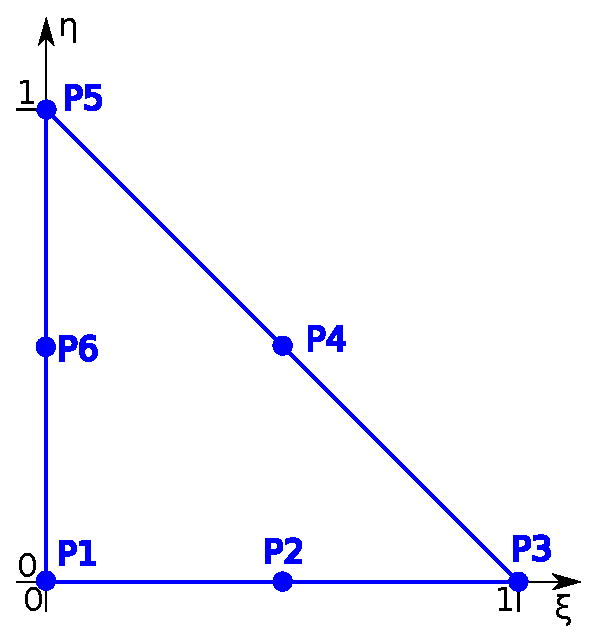
\includegraphics[scale=0.65]{pics/quadratic_element.eps}
	\end{center}
	\caption{Ansatz für quadratisches Element}
	\label{fig:quadratic_element}
\end{wrapfigure}

Der Ansatz der Potentialfunktion wird wie folgt gewählt:
\begin{equation}
\label{eq:quadratic_triangle_eq}
u(\xi, \eta) = c_0 + c_1 \xi + c_2 \eta + c_3 \xi \eta + c_4 \xi^2 + c_5 \eta^2
\end{equation}	
Nach dem Einsetzen der Knotenkoordinaten ergeben sich folgende Gleichungen zur Bestimmung der Unbekannten $c_j$:
\begin{align}
&u(0,0) = u_1 = c_0\\
&u(\nicefrac{1}{2}, 0) = u_2 = c_0 + \frac{1}{2} c_1 + \frac{1}{4} c_4 \nonumber \\
&u(1, 0) = u_3 = c_0 + c_1 + c_4 \nonumber \\
&u(\nicefrac{1}{2}, \nicefrac{1}{2}) = u_4 = c_0 + \frac{1}{2} c_1 + \frac{1}{2} c_2 + \frac{1}{4} c_3 + \frac{1}{4} c_4  \nonumber \\ 
&\quad \quad \quad \quad \quad \quad \quad \quad \ +\frac{1}{4} c_5\nonumber \\
&u(0, 1) = u_5 = c_0 + c_2 + c_5 \nonumber \\
&u(\nicefrac{1}{2}, 0) = u_6 = c_0 + \frac{1}{2} c_2 + \frac{1}{4} c_5 \nonumber
\end{align}		

Durch Anwendung des gleichen Prinzips wie in Abschnitt \ref{sec:linear_triangles} können nun die Formfunktionen $N_1 \text{...} N_6$ ermittelt werden. Diese finden sich in Anhang ... .




% =============================== Kubische Elemente ======================================

\subsubsection{Kubische Dreieckselemente}

Das kubische isoparametrische finite Dreieckselement ist wie in Abbildung \ref{fig:cubic_element} definiert.

\begin{wrapfigure}{r}{8cm}
	\vspace{-6cm}
	\begin{center}
		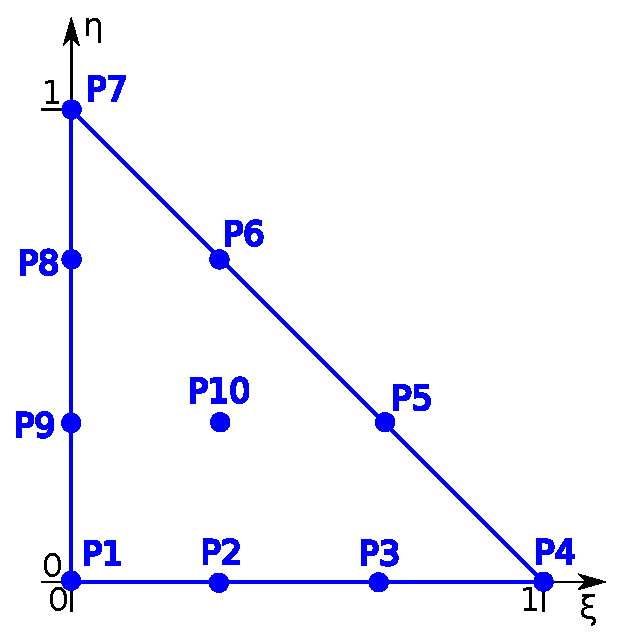
\includegraphics[scale=0.65]{pics/cubic_element.eps}
	\end{center}
	\caption{Ansatz für quadratisches Element}
	\label{fig:cubic_element}
\end{wrapfigure}

Die Koordinaten der drei Elementknoten lauten wie folgt:
\begin{align}
&P_1 = \coord{0}{0}, \quad P_2 = \coord{\nicefrac{1}{3}}{0}\\
&P_3 = \coord{\nicefrac{2}{3}}{0}, \quad P_4 = \coord{1}{0} \nonumber \\
&P_5 = \coord{\nicefrac{2}{3}}{\nicefrac{1}{3}}, \quad P_6 = \coord{\nicefrac{1}{3}}{\nicefrac{2}{3}} \nonumber\\
&P_7 = \coord{0}{1}, \quad P_8 = \coord{0}{\nicefrac{2}{3}} \nonumber \\
&P_9 = \coord{0}{\nicefrac{1}{3}}, \quad P_10 = \coord{\nicefrac{1}{3}}{\nicefrac{1}{3}} \nonumber\\
\end{align}

Der Ansatz der Potentialfunktion wird wie folgt gewählt:

\begin{equation}
\label{eq:cubic_triangle_eq}
u(\xi, \eta) = c_0 + c_1 \xi + c_2 \eta + c_3 \xi \eta + c_4 \xi^2 + c_5 \eta^2 + c_6 \xi^2 \eta + c_7 \xi \eta^2 + c_8 \xi^3 + c_9 \eta^3
\end{equation}	



Nach dem Einsetzen der Knotenkoordinaten ergeben sich folgende Gleichungen zur Bestimmung der Unbekannten $c_j$:
\begin{align}
u(0,0) = &u_1 = c_0\\
u(\nicefrac{1}{3}, 0) = &u_2 = c_0 + \frac{1}{3} c_1 + \frac{1}{9} c_4 +  \frac{1}{27} c_8\nonumber \\
u(\nicefrac{2}{3}, 0) = &u_3 = c_0 + \frac{2}{3} c_1 + \frac{4}{9} c_4 +  \frac{8}{27} c_8\nonumber \\
u(1,0) = &u_4 = c_0 + c_1 + c_4 + c_8\nonumber\\
u(\nicefrac{2}{3}, \nicefrac{1}{3}) = &u_5 = c_0 + \frac{2}{3} c_1 +  \frac{1}{3} c_2 + \frac{2}{9} c_3 +  \frac{4}{9} c_4 + \frac{1}{9} c_5 + \frac{4}{27} c_6 + \frac{2}{27} c_7 + \frac{8}{27} c_8 + \frac{1}{27} c_9\nonumber\\
u(\nicefrac{1}{2}, 0) = &u_6 = c_0 + \frac{1}{3} c_1 +  \frac{2}{3} c_2 + \frac{2}{9} c_3 +  \frac{1}{9} c_4 + \frac{4}{9} c_5 + \frac{2}{27} c_6 + \frac{4}{27} c_7 + \frac{1}{27} c_8 + \frac{8}{27} c_9\nonumber\\
u(0,1) = &u_7 = c_0 + c_2 + c_5 + c_9\nonumber\\
u(0, \nicefrac{2}{3}) = &u_8 = c_0 + \frac{2}{3} c_2 + \frac{4}{9} c_5 +  \frac{8}{27} c_9\nonumber \\
u(0, \nicefrac{1}{3}) = &u_9 = c_0 + \frac{1}{3} c_2 + \frac{1}{9} c_5 +  \frac{1}{27} c_9\nonumber \\
u(\nicefrac{1}{3}, \nicefrac{1}{3}) = &u_{10} = c_0 + \frac{1}{3} c_1 +  \frac{1}{3} c_2 + \frac{1}{9} c_3 +  \frac{1}{9} c_4 + \frac{1}{9} c_5 + \frac{1}{27} c_6 + \frac{1}{27} c_7 + \frac{1}{27} c_8 + \frac{1}{27} c_9\nonumber
\end{align}	
	

Durch Anwendung des gleichen Prinzips wie in Abschnitt \ref{sec:linear_triangles} können nun die Formfunktionen $N_1 \text{...} N_10$ ermittelt werden. Diese finden sich in Anhang ... .
\subsection{Problemtypen}
In diesem Kapitel werden die in der Software implementierten Problemtypen beschrieben. In beiden Fällen handelt es sich um zweidimensionale, ebene Probleme. Resultat dieses Abschnitts werden analytische Berechnungsvorschriften für die einzelnen Elementgleichungssysteme sein.\newline
Die Berechnungen aus diesem Abschnitt stammen, sofern nicht anders angegeben, aus \cite{SMS_VO_skript} Kapitel 7 und 8. Für ausführliche Herleitungen, auf welche in diesem Fall bewusst verzichtet wird, sei auf das oben genannte Werk verwiesen.\newline

Wie aus Abschnitt \ref{sec:fem_theory} bekannt, ist das Randwertproblem zuerst als Operatorgleichung mit entsprechenden Randwertbedingungen zu formulieren. Die Operatorgleichung kann nun entweder direkt im Galerkinschen Verfahren oder über Umweg eines äquivalenten Funktionals im Ritzschen Verfahren verwendet werden. Dabei wird für die gesuchte Funktion $u$ in jedem Teilgebiet (finites Element) ein entsprechender Approximations-Ansatz wie in Abschnitt \ref{sec:finite_elements_and_shape_functions} ermittelt, eingesetzt. Das Ergebnis sind 'lokale' lineare Gleichungssysteme (für jedes Element eines), welche zu einem großen, 'globalen' Gleichungssystem assembliert werden müssen. Auf die Assemblierung wird dabei genauer in Abschnitt \ref{sec:assembling} eingegangen.\newline

Ausgangspunkt für Probleme aus der Elektrotechnik sind im Allgemeinen die Maxwell-Gleichungen:
\begin{align}
	\mathit{rot}\vec{E} = -\parDiff{\vec{B}}{t} \label{eq:maxwell_1} \\
	\mathit{rot}\vec{H} = \vec{J} + \parDiff{\vec{D}}{t} \label{eq:maxwell_2}\\
	\mathit{div}\vec{B} = 0 \label{eq:maxwell_3}\\
	\mathit{div}\vec{D} = \rho \label{eq:maxwell_4}
\end{align}
mit den Materialzusammenhängen
\begin{align}
\vec{D} = [\epsilon]\vec{E} \label{eq:material_1}\\
\vec{B} = [\mu]\vec{H} \label{eq:material_2}
\end{align}
mit $[\epsilon]$ und $[\mu]$ als ortsabhängigen Materialtensoren.

\subsubsection{Elektrostatische Probleme}
\label{sec:electrostatic_problems}
Für den elektrostatischen Fall ist $\vec{J},\ \vec{H}$, sowie sämtliche zeitlichen Änderungen $\equiv 0$ wodurch sich $\vec{B}$ sowie die rechte Seite von (\ref{eq:maxwell_1}) zu $\equiv 0$ ergeben.\newline
Ein elektrostatisches Problem wird somit durch die folgenden Gleichungen beschrieben:
\begin{align}
\mathit{rot}\vec{E} &= 0 \label{eq:wirbelfreiheit_E}\\
\mathit{div}\vec{D} &= \rho \label{eq:sources_D}
\end{align}\newline

Aufgrund der Wirbelfreiheit des elektrischen Feldes aus (\ref{eq:wirbelfreiheit_E}) kann nun folgender Ansatz für die elektrische Feldstärke $\vec{E}$ verwendet werden:
\begin{equation}
\label{eq:dgl_E}
\vec{E} = -\mathit{grad}V
\end{equation}
mit $V$ als sogenanntem \textit{Skalapotential}.\newline

Setzt man (\ref{eq:dgl_E}) nun unter Verwendung von (\ref{eq:material_1}) in (\ref{eq:sources_D}) ein, so erhält man die partielle Differentialgleichung für $V$ als:
\begin{equation}
\mathit{div}[\epsilon]\mathit{grad}V = -\rho
\end{equation}
Hierbei entspricht $\mathit{div}[\epsilon]\mathit{grad}$ dem Differentialoperator $L$ aus (\ref{eq:operatorgleichung}), das Potential $V$ der gesuchten Funktion $u$ und $-\rho$ der gegebenen Funktion $f$.\newline

Die Randbedingungen für ein solches Problem sind gegeben als
\begin{equation}
\label{eq:e-static_dirichlet_condition}
	V = \overline{V}
\end{equation}
am dirichletschen Rand $\Gamma_D$ und 
\begin{equation}
\label{eq:e-static_neumann_condition}
\vec{n}\cdot\mathit{grad}V = \sigma 
\end{equation}
am neumannschen Rand $\Gamma_N$, mit $\vec{n}$ als Flächennormale und $\sigma$ als gegebener Flächenladungsdichte.\newline

Unter Verwendung des Ritzschen \textit{oder} Galerkinschen Verfahrens erhält man nun Formeln zur Berechnung der Elementgleichungssysteme, wobei beide Verfahren dieselben (!) Formeln liefern. Löst man (\ref{eq:first_variation}) oder (\ref{eq:weighted_residuum}) mit den entsprechenden Ansätzen, so ergibt sich für jedes Element ein quadratisches lineares \textit{Elementgleichungssystem} $\begin{bmatrix}k_{ij}\end{bmatrix} \cdot \begin{Bmatrix}V_j\end{Bmatrix} = \begin{Bmatrix}r_j\end{Bmatrix}$ der Dimension $N\times N$ mit $N$ als Anzahl der Elementknoten.
\begin{equation}
\label{eq:k_ij_e_static}
k_{ij} = \int\displaylimits_{x} \int\displaylimits_{y} \left(\epsilon_x \parDiff{N_i}{x}\parDiff{N_j}{x} +  \epsilon_y\parDiff{N_i}{y}\parDiff{N_j}{y}\right)dx dy
\end{equation}


\begin{equation}
\label{eq:right_side_e_static}
	r_j = \int\displaylimits_{x} \int\displaylimits_{y} N_i \rho dx dy + \int\displaylimits_{\Gamma_N} N_i\sigma d\Gamma
\end{equation}

\textbf{Anmerkung:} Um auf die oben gezeigte Form für $k_ij$ zu kommen ist es notwendig den Permettivitätstensor $[\epsilon]$ auf die Hauptachsenform zu transformieren:
\begin{equation*}
	[\epsilon] = \begin{bmatrix}
	\epsilon_x & 0 \\
	0 & \epsilon_y
	\end{bmatrix}
\end{equation*}

Man beachte dass für Formfunktionen von isoparametrischen finite Elementen $N_i = N_i(\xi, \eta)$ gilt, wodurch alle Integrale in den Variablen $\xi$ und $\eta$ durchgeführt werden müssen. Die entsprechende Substitution sowie die Realisierung der Integrale werden in Abschnitt \ref{sec:equation_system_calculation} genauer behandelt. 


\subsubsection{Stationäre Strömungsfeldprobleme}
\label{sec:stat_current_problems}
Stationäre Strömungsfeldprobleme lassen sich über das Gesetz der Ladungserhaltung definieren:
\begin{equation}
	\mathit{div}\vec{J} = 0
\end{equation}
 Es muss außerdem das Ohmsche Gesetz in seiner differentiellen Form gelten:
 \begin{equation}
 	\vec{J} = [\gamma] \vec{E}
 \end{equation}
 mit $[\gamma]$ als ortsabhängigem Tensor der spezifischen Leitfähigkeit.\newline
 
 Stationäre Strömungsfeldprobleme können somit analog zu elektrostatischen Problemen mittels folgender Differentialgleichung ermittelt werden:
 \begin{equation}
\mathit{div}[\gamma]\mathit{grad}V = 0
 \end{equation}
 Als Randbedingungen ergeben sich:
 \begin{equation}
 \label{eq:current_dirichlet_condition}
 V = \overline{V}
 \end{equation}
 am dirichletschen Rand $\Gamma_D$ und 
 \begin{equation}
 \label{eq:current_neumann_condition}
 \vec{n}\cdot\mathit{grad}V = J_e
 \end{equation}
 am neumannschen Rand $\Gamma_N$, wobei $J_e$ die eingeprägte Flächenstromdichte am Rand darstellt.\newline
 
 Man erkennt die starken Äquivalenzen zwischen stationären Strömungsfeldproblemen und elektrostatischen Problemen. Das Elementgleichungssystem ergibt sich somit für diese Probleme als
 
\begin{equation}
\label{eq:k_ij_stat_current}
k_{ij} = \int\displaylimits_{x} \int\displaylimits_{y} \left(\gamma_x \parDiff{N_i}{x}\parDiff{N_j}{x} +  \gamma_y\parDiff{N_i}{y}\parDiff{N_j}{y}\right)dx dy
\end{equation}

\begin{equation}
\label{eq:right_side_stat_current}
r_j = \int\displaylimits_{x} \int\displaylimits_{y} N_i J_e dx dy
\end{equation}



\subsubsection{Berechnung der Elementmatrix-Koeffizienten $k_{ij}$}

Da die Formfunktionen $N_i$ bei isoparametrischen finiten Elementen Funktionen von $\xi$ und $\eta$ sind, müssen die Integrationsvariablen aller Integrale substituiert werden.  \newline
Die partiellen Ableitungen der Formfunktionen, wie sie z.B. in (\ref{eq:k_ij_e_static}) benötigt werden, ergeben nach \cite{SMS_VO_skript}, S.72 aus
\begin{equation}
\begin{Bmatrix}
\parDiff{N}{\xi} \\[2mm]
\parDiff{N}{\eta}
\end{Bmatrix} = 
\underbrace{
\begin{bmatrix}
\sum\limits_{k}\parDiff{N_k}{\xi}x_k & \sum\limits_{k}\parDiff{N_k}{\xi}y_k \\[2mm]
\sum\limits_{k}\parDiff{N_k}{\eta}x_k & \sum\limits_{k}\parDiff{N_k}{\eta}y_k
\end{bmatrix}}_{\mat{J}}\cdot
\begin{Bmatrix}
\parDiff{N}{x} \\[2mm]
\parDiff{N}{y}
\end{Bmatrix}
\end{equation}
zu
\begin{equation}
\label{eq:partial_derivatives_subst}
\begin{Bmatrix}
\parDiff{N}{x} \\[2mm]
\parDiff{N}{y}
\end{Bmatrix} = 
\underbrace{
	\frac{1}{\mathit{det}(\mat{J})}\begin{bmatrix}
	 \sum\limits_{k}\parDiff{N_k}{\eta}y_k & -\sum\limits_{k}\parDiff{N_k}{\xi}y_k \\[2mm]
	-\sum\limits_{k}\parDiff{N_k}{\eta}x_k & \sum\limits_{k}\parDiff{N_k}{\xi}x_k
	\end{bmatrix}}_{\mat{J}^{-1}}
\cdot \left\{ \begin{matrix}
\parDiff{N}{\xi} \\[2mm]
\parDiff{N}{\eta}
\end{matrix} \right\}_{.}
\end{equation}


Das Flächenelement $dxdy$ in (\ref{eq:k_ij_e_static}) ergibt sich mit den Beziehungen aus \cite{SMS_VO_skript}, S.74 zu 
\begin{equation}
\label{eq:surface_element}
dxdy = \mathit{det} \mat{(J)} d\xi d\eta,
\end{equation}
wobei das Flächenintegral in beiden Koordinaten in den Intervallen $\xi \in [0,1], \ \eta \in [0, 1-\xi]$ durchzuführen ist. Somit ergibt sich der Elementmatrix-Koeffizient $k_{ij}$ zu 
\begin{align}
&k_{i,j} = \int\displaylimits_{\xi = 0}^{1} \int\displaylimits_{\eta = 0}^{1 - \xi} \bigg[\\
%
% x-derivatives
&\frac{\epsilon_x}{\mathit{det}(\mat{J})}\left(\parDiff{N_i}{\xi}\sum\limits_{k}\parDiff{N_k}{\eta}y_k - \parDiff{N_i}{\eta}\sum\limits_{k}\parDiff{N_k}{\xi}y_k\right)
%
\left(\parDiff{N_j}{\xi}\sum\limits_{k}\parDiff{N_k}{\eta}y_k - \parDiff{N_j}{\eta} -\sum\limits_{k}\parDiff{N_k}{\xi}y_k\right) + \nonumber\\ 
%
% y-derivatives
&\frac{\epsilon_y}{\mathit{det}(\mat{J})}\left(-\parDiff{N_i}{\xi}\sum\limits_{k}\parDiff{N_k}{\eta}x_k + \parDiff{N_i}{\eta} \sum\limits_{k}\parDiff{N_k}{\xi}x_k\right)
%
\left(-\parDiff{N_j}{\xi}\sum\limits_{k}\parDiff{N_k}{\eta}x_k + \parDiff{N_j}{\eta} \sum\limits_{k}\parDiff{N_k}{\xi}x_k\right) \nonumber\\ 
& \bigg]d\xi d\eta
\end{align}

\textbf{Anmerkung:} Man beachte dass das $\mathit{det}(\mat{J})$ des Flächenelements aus (\ref{eq:surface_element}) bereits gekürzt wurde.\newline
Die Berechnung der partiellen Ableitungen der Formfunktionen kann auf analytischem Wege vorweg erfolgen, da diese nur vom gewählten Elementtyp abhängen. Somit ist eine effiziente Berechnung der Terme $\sum\limits_{k}\parDiff{N_k}{\eta}y_k$ in Form von Skalarprodukten möglich.\newline


\subsubsection{Berechnung der Rechtsseiten-Elemente $r_j$}
Die Berechnung der Koeffizienten der 'rechten Seite' eines elektrostatischen Problems 
\begin{equation}
r_j = \int\displaylimits_{x} \int\displaylimits_{y} N_i \rho dx dy + \int\displaylimits_{\Gamma_N} N_i\sigma d\Gamma
\end{equation}
erfordert zu einen ein Flächenintegral (erster Summand) und ein Integral über den neumannschen Rand, welches im zweidimensionalen Fall zu einem Kurvenintegral entartet. \newline
Für das Flächenintegral lässt sich die Substitution der Integrationsvariablen sehr einfach durchführen, da keine partiellen Ableitungen des Formfunktionen vorkommen:
\begin{equation}
\int\displaylimits_{x} \int\displaylimits_{y} N_i \rho dx dy = \int\displaylimits_{\xi = 0}^{1} \int\displaylimits_{\eta = 0}^{1 - \xi} N_i \rho \mathit{det} (\mat{J}) d\xi d\eta.
\end{equation}
\newline

Für Kurvenintegral über den neumannschen Rand ändert sich der Integrand je nach dem über welche Dreiecksseite integriert wird. 
Das entartete Flächenintegral über den neumannschen Rand hat nun folgende Form:
\begin{equation}
	\int\displaylimits_{c}N_i(\xi, \eta)\sigma ds.
\end{equation}

Allgemein gilt (siehe \cite{SMS_VO_skript}, S. 74f.):
\begin{align}
\label{eq:subs}
\vec{d\xi} = dx\vec{e_x} + dy\vec{e_y} = \parDiff{x}{\xi}d\xi \vec{e_x} + \parDiff{x}{\xi} d\xi \vec{e_y},\\
\vec{d\eta} = dx\vec{e_x} + dy\vec{e_y} = \parDiff{x}{\eta}d\eta \vec{e_x} + \parDiff{x}{\eta} d\eta \vec{e_y} .\nonumber
\end{align}
Das infinitesimale Kurvenelement ergibt sich somit nun zu $\vec{ds} = \vec{d\xi} + \vec{d\eta}$ bzw. \begin{equation}
\label{eq:ds_abs}
ds = \left|\left| \vec{ds} \right|\right| = \sqrt{\left(\vec{d\xi} + \vec{d\eta}\right)^T\cdot \left( \vec{d\xi} + \vec{d\eta} \right)}.
\end{equation}\newline

Integriert man über die Dreiecksseite 1, so gilt $d\eta = 0$ und somit auch $\vec{d\eta} = \vec{0}$.
Somit gilt für $\vec{ds}$ bzw. $ds$ unter Verwendung von (\ref{eq:ansatz_isoparam}):
\begin{align}
	&\vec{ds} =  \vec{d\xi} \Rightarrow \nonumber \\
	&ds = \left|\left| \vec{d\xi} \right|\right| = \sqrt{ \left(\parDiff{x}{\xi}\right)^2 + \left(\parDiff{y}{\xi}\right)^2} d\xi = \sqrt{ \left( \sum\limits_{k}\parDiff{N_k}{\xi}x_k \right)^2  + \left( \sum\limits_{k}\parDiff{N_k}{\xi}y_k \right)^2 } d\xi
\end{align}

Selbiges kann für Dreiecksseite 2 unter Verwendung von $d\xi = 0$ hergeleitet werden. Es ergibt sich somit:
\begin{align}
&\vec{ds} =  \vec{d\eta} \Rightarrow \nonumber \\
&ds = \left|\left| \vec{d\eta} \right|\right| = \sqrt{ \left(\parDiff{x}{\eta}\right)^2 + \left(\parDiff{y}{\eta}\right)^2} d\eta = \sqrt{ \left( \sum\limits_{k}\parDiff{N_k}{\eta}x_k \right)^2  + \left( \sum\limits_{k}\parDiff{N_k}{\eta}y_k \right)^2 } d\eta
\end{align}

Zur Integration über Dreiecksseite 3  muss zuerst die Kurve parametrisiert werden:
\begin{align*}
&\vec{s(t)} = 
\begin{Bmatrix}
\xi(t) \\ \eta(t)
\end{Bmatrix} = 
\begin{Bmatrix}
1 - t \\ t
\end{Bmatrix} \Rightarrow\\
%
&\frac{ds}{dt} = 
\begin{Bmatrix}
\frac{d\xi}{dt} \\ \frac{d\eta}{dt}
\end{Bmatrix} = 
\begin{Bmatrix}
-1 \\ 1
\end{Bmatrix} \Rightarrow \\
% 
&\underline{\underline{d\xi = -dt, \ d\eta = dt}}
\end{align*}

Setzt man dies nun in (\ref{eq:subs}) und dies wiederum in (\ref{eq:ds_abs}) ein, so erhält man
\begin{equation}
ds = \sqrt{\left(\parDiff{x}{\eta} - \parDiff{x}{\xi}\right)^2  + \left(\parDiff{y}{\eta} - \parDiff{y}{\xi}\right)^2} dt
\end{equation}

Setzt man nun für $x$ und $y$ die entsprechenden Zusammenhänge aus (\ref{eq:ansatz_isoparam}) ein erhält man:
\begin{equation}
ds = \sqrt{  \left(  \sum\limits_{k}\parDiff{N_k}{\eta}x_k  - \sum\limits_{k}\parDiff{N_k}{\xi}x_k  \right)^2 + \left(  \sum\limits_{k}\parDiff{N_k}{\eta}y_k  - \sum\limits_{k}\parDiff{N_k}{\xi}y_k  \right)^2  } dt
\end{equation}



\section{Implementierung}
Dieses Kapitel beschäftigt sich mit diversen Details der Implementierung des finite Elemente Algorithmus in der Software. Es wird beschrieben wie mittels der Software Gmsh die Problemgeometrie erstellt, sowie ein finite Elemente Gitter generiert und exportiert wird. Anschließend erfolgt ein kurzer Umriss des Imports und Verarbeitung des Gitters zur Verwendung im eigentlichen Lösungsalgorithmus auf den detaillierter am Ende dieses Kapitels eingegangen wird.
\subsection{Erstellung der Geometrie und Generierung des Gitters mit Gmsh}
\subsubsection{Erstellung der Geometrie}
Die Erstellung der Geometrie sowie die Generierung des FEM-Gitters erfolgt mit der Open-Source Software Gmsh. \cite{gmsh_website}
Gmsh stellt zwei CAD-Kernel ('Built-In' und 'OpenCASCADE') zur Verfügung welche jedoch sehr ähnlich zu Bedienen sind. Auf Unterschiede wird entsprechend hingewiesen.\newline

Gmsh nutzt dabei eine eigene Skript-Sprache zur Erstellung der Geometrie, wobei die einzelnen Kommandos für den jeweiligen CAD-Kernel übersetzt werden. Eine Geometrie in Gmsh wird also durch ein ASCII-codiertes File mit einer Sequenz von Kommandos repräsentiert. Ein Beispiel für ein einfaches Viereck ist in Abbildung ... gezeigt. Die Erstellung der Geometrie erfolgt dabei 'Bottom-Up'. Dabei werden zuerst Punkte im Raum festgelegt, welche dann durch Linien verbunden werden. Mehrere aneinander grenzende Linien bilden eine Fläche und mehrere aneinander grenzende Flächen ein Volumen. Für eine genauere Beschreibung des Ablaufs sei auf die sehr ausführliche Dokumentation auf der Gmsh-Homepage verwiesen (\cite{gmsh_website}).\newline

Eine besondere Rolle bei der Erstellung der Problemgeometrie nehmen die sogenannten 'Physical Groups' ein. Wie ihr Name schon sagt, sind dies Gruppen von Elementen (z.B. Linien) mit der gleichen physikalischen Eigenschaft. (z.B. dem gleichen Potential). Um dies besser zu erklären ist in Abbildung ... die Problemgeometrie eines einfachen Plattenkondensators dargestellt. Die Linien die die obere Elektrode bilden wurden zu einer 'Physical Group' mit dem Namen 'dir100' zusammengefügt. Später wird diese geschlossene Kurve als dirichletscher Rand mit einer Bedingung von $V = 100$ deklariert. Das äußere Viereck dient als ferner Rand mit einer dirichletschen Randbedingung von $V=0$ und wird daher ebenfalls zu einer 'Physical Group' mit dem Namen 'farbound' zusammengefasst. Ebenso wird der Rand der unteren Elektrode zu einer Gruppe mit dem Namen 'dir0' zusammengefasst.
 zusammengefasst.\newline
 Auch Flächen können zu 'Physical Groups' zusammengefasst werden. Typischerweise sind dies Areale mit den gleichen Materialeigenschaften (Permettivität) und/oder gleichen Quellen (freie Raumladungen). In dem gezeigten Beispiel gibt es drei sogenannte 'Physical Surfaces', eine welche den Bereich der umschließenden Luft modelliert, und zwei zur Modellierung eines geschichteten Dielektrikums zwischen den Kondensatorplatten.
 
 \subsubsection{Generierung des Gitters}
 Gmsh erlaubt die Verwendung von verschiedenen Algorithmen zur Gittergenerierung. In der Standardeinstellung wählt Gmsh automatisch einen geeigneten Algorithmus aus, wobei sich dies als völlig zufriedenstellend herausgestellt hat. Wie schon bei der Geometrie, erfolgt die Generierung des Gitters 'Bottom-Up' wobei zuerst Linen, dann Flächen und schließlich Volumen bearbeitet werden. Ein simpler Klick auf \textit{Mesh $\rightarrow$ 2D} führt alle genötigten Schritte durch, wobei standardmäßig ein lineares, 3-knotiges Dreiecksgitter erzeugt wird. Zum Wechsel auf ein Gitter höherer Ordnung ist ein Kick auf \textit{Mesh $\rightarrow$ Set order<n>} nötig, wobei <n> für die gewünschte Gitterordnung steht. Um das bestehende Gitter zu verfeinern, muss lediglich auf \textit{Mesh $\rightarrow$ Refine by splitting} geklickt werden. Bei unpassender Aufteilung des verfeinerten Gitters empfiehlt sich ein erneuter Klick auf \textit{Mesh $\rightarrow$ 2D} wodurch sich die Aufteilung der Elemente wieder verbessern sollte.\newline
 
 Zum Export des Gitters ist folgender Ablauf zu befolgen:
 \begin{itemize}
 	\item \textit{File $\rightarrow$ Export}
 	\item Auswahl des Ordners und Dateinamens \textbf{mit der Endung .msh} (Gmsh erkennt des Typ der zu Exportierenden Datei anhand seiner Endung)
 	\item Auswahl der 'Version 2' unter den anschließend angezeigten Optionen
 \end{itemize}

\textbf{Anmerkung:} Ein simpler Export mittels \textit{File $\rightarrow$ Save mesh} ist nicht möglich, da Gmsh dann das Gittern in einer .msh-Datei der Version 4 abspeichert, das FEM-Tool jedoch nur Version 2 unterstützt.\newline

\textbf{Anmerkung:} Die Generierung des Gitters kann auch automatisiert im FEM-Tool erfolgen. Somit ist ein händischer Export nur nötig wenn spezielle Änderungen am Gitter von Hand vorgenommen werde müssen.

\subsection{Import und Verarbeitung des FEM-Gitters}
In diesem Abschnitt wird kurz der Import und die Verarbeitung des FEM-Gitters beschrieben. Dabei wird genauer auf die Methodik zur korrekten Interpretation der Randbedingungen eingegangen. So erfordert zum Beispiel die Berechnung des Elementgleichungssystems im 2D-Fall ein Kurvenintegral entlang des neumannschen Randes, wobei sich diese aus mehreren Dreiecksseiten zusammensetzt. Somit ist es zwingend notwendig aus dem generierten Gitter herauszulesen welche Seite oder Seiten der entsprechenden Elemente am neumannschen Rand liegen.

\subsubsection{Import des Gitters}
Wie schon zuvor erwähnt benötigt die Software eine Gitterdatei der Version 2. Dabei handelt es sich um ASCII-codierte Dateien mit \textbf{mindestens} folgenden Informationen:

\begin{itemize}
	\item \textbf{Format der Datei im Abschnitt \textit{\$MeshFormat\$}}. Sie Software unterstützt nur Dateien der Version 2.2.0.8
	
	\item \textbf{Informationen über die 'Physical Groups' der Problemgeometrie im Abschnitt \textit{\$Physical Names\$}}. Dabei gibt der erste Eintrag des Abschnitts die Anzahl der \textit{Physical Groups} an. Jeder weitere Eintrag steht für eine \textit{Physical Group}, definiert durch jeweils drei Parameter:
	\begin{enumerate}
		\item \textbf{Dimension der \textit{Physical Group}}. 1: 1-dimensional (Kurve), 2: 2-dimensional (Fläche)
		\item \textbf{ID}. Jede Gruppe bekommt eine positive Ganzzahl zur eindeutigen Identifikation zugewiesen.
		\item \textbf{Name}. Jener Name der der \textit{Physical Group} bei der Erstellung zugewiesen wurde.
	\end{enumerate}

	\item \textbf{Daten der Elementkonten des Gitters im Abschnitt \textit{\$Nodes\$}}. Der erste Eintrag gibt wieder die Anzahl der Knoten an, jeder weitere Eintrag steht für einen Knoten, wobei die erste Zahl eine positive Ganzzahl zur eindeutigen Identifizierung des Knotens darstellt. Die weiteren drei Einträge sind Gleitkommazahlen für die x-, y- und z-Koordinaten.
	
	\item \textbf{Definitionen der finiten Elemente im Abschnitt \textit{\$Elements\$}}. Der erste Eintrag gibt die Anzahl der finiten Elemente an, und jede weiter Zeile definiert ein Element nach dem folgenden Schema:
	\begin{enumerate}
		\item \textbf{ID}. Eine positive Ganzzahl zur eindeutigen Identifikation des Elements.
		\item \textbf{Typ des Elements}. Gmsh kennt viele verschiedene Elementtypen. Für eine vollständige Liste sei auf die Dokumentation von Gmsh verwiesen (\cite{gmsh_website}). Da sie Software dreieckige finite Elemente bis zur Ordnung 3 unterstützt sind hier folgende Einträge möglich:
		\begin{itemize}
			\item 2: 2-knotige lineare Linie/Kurve
			\item 3: 3-knotiges lineares Dreieckselement
			\item 8: 3-knotige quadratische Line/Kurve
			\item 9: 6-knotiges quadratisches Dreieckselement
			\item 26: 4-knotige kubische Linie/Kurve
			\item 21: 10-knotiges kubisches Dreieckselement
		\end{itemize}
		\textbf{Anmerkung:} In Zukunft könnten weitere Elementtypen unterstützt werden.
		\item \textbf{Anzahl der \textit{Physical Tags}}. 
		\item 'Physical Tage'. Auch hier sei zu deren genauen Bedeutung auf die Dokumentation von Gmsh \cite{gmsh_website} verwiesen. Standardmäßig ist der erste Eintrag nach der Anzahl der \textit{Physical Tags} die ID der \textit{Physical Group} der das Element angehört. Alle Weiteren \textit{Tags} werden nicht benötigt.
		\item \textbf{IDs der Elementknoten}. Je nach Elementtyp findet sich hier eine unterschiedliche Anzahl an Einträgen. Es ist zu beachten dass Gmsh die Reihenfolge der Knoten der finiten Elemente anders als das FEM-Tool definiert. Hierbei sei auf die Gmsh Dokumentation, Abschnitt 9.2 verwiesen. Die Definitionen des FEM-Tools finden sich in diesem Dokument unter Abschnitt \ref{sec:finite_elements_and_shape_functions}. Es ist somit ein Umordnen der Knoten notwendig, was jedoch von der Software automatisch beim Import durchgeführt wird.
	\end{enumerate}
\end{itemize}

Eine Beispielhafte Gitterdatei zu dem in Abbildung \ref{fig:neumann_boundary_assignment} gezeigten Beispiel findet sich in Code \ref{fig:example_mesh_file}.


\subsubsection{Verarbeitung der Gitterinformation}
Nach erfolgreichem Import der Gitterinformation ist als letzter Schritt or der eigentlichen Lösung nun notwendig die Randbedingungen des Problems, sowie Materialeigenschaften und weitere Informationen wie zum Beispiel Quellen (freie Raumladungen etc.) den einzelnen Elementen zuzuordnen: \newline

\begin{itemize}
	\item \textbf{Knoten am dirichletschen Rand}. Das Potential des entsprechenden Elementknotens ist bereits vorgegeben, was bei der Berechnung des Elementgleichungssystems entsprechend berücksichtigt werden muss.
	\item \textbf{Knoten und Seiten am neumannschen Rand}. Wie aus (\ref{eq:right_side_e_static}) ersichtlich erfordert die Berechnung von $r_j$ ein Integral über die neumannsche Randfläche, welches im zweidimensionalen Fall zu einem Kurvenintegral entartet. Dazu ist es notwendig zu wissen welche Dreiecksseiten der Elemente am neumannschen Rand liegen.
	\item \textbf{Materialeigenschaften im Element}. Wie in \ref{eq:k_ij_e_static} ersichtlich ist es notwendig $\epsilon_x$ und $\epsilon_y$ für jedes Element zu kennen. Die Deklaration von $\epsilon_x$ und $\epsilon_y$ erfolgt in einem separaten File. Die Zuordnung zum entsprechenden Element erweist sich als trivial da jeder Elementdefinition die ID der entsprechenden 2D \text{Physical Group} beiliegt.
	\item \textbf{Quellen im Element}. Analog zu den Materialeigenschaften verhält es sich mit den Quellen innerhalb eines Elements. Die Quellen kommen z.B. bei der Berechnung von (\ref{eq:right_side_e_static}) als Parameter $\rho$ zum Tragen. Auch hier erweist sich die Zuordnung wieder als trivial.
\end{itemize}

Die Zuordnung der Knoten und Dreiecksseiten an den Rändern des Problems wird im folgenden Kapitel beschrieben.

\subsubsection{Zuordnung der Knoten am dirichletschen- und Dreiecksseiten am neumannschen Rand}
\label{sec:rb_assignment}
\textbf{Knoten am dirichletschen Rand:}
\begin{enumerate}
	\item Man ermittle alle Elementknoten am gewählten Rand aus den dem Rand zugeordneten Kurvenelementen. Da die Definition der Kurvenelemente in der Gitterdatei bereits die ID der entsprechenden \textit{Physical Group} enthält ist diese Aufgabe trivial.
	\item Man suche nun alle Dreieckselemente die mindestens einen der vorher ermittelten Knoten beinhalten und speichere diese Zuordnung samt Randwerte für die entsprechenden Knoten.
\end{enumerate}

\textbf{Dreiecksseiten am neumannschen Rand:}
\begin{enumerate}
	\item Man wende den gleichen Algorithmus wie oben an.
	\item Man ermittle die Dreiecksseite am neumannschen Rand durch Vergleich der Rand- und Elementknoten:\newline
	Je nach Elementtyp ist eine Dreiecksseite durch 2, 3 oder 4 Knoten definiert. Siehe dazu Abschnitt \ref{sec:finite_elements_and_shape_functions}. Liegt ein Dreieckselement am neumannschen Rand, so stimmen alle Knoten einer oder mehrerer Seiten mit entsprechend vielen Knoten am Rand überein. Hierbei ist zu erwähnen dass auch bei mehr als 2 Knoten pro Seite immer nur eine ganze Seite am Rand liegen kann. \newline
	Durch die Verwendung von isoparametrischen finiten Elementen sind im lokalen Koordinatensystem nur drei verschiedene Kurvenintegrale möglich, was eine statische Zuordnung eines Kurvenintegrals zu jeder Dreiecksseite ermöglicht. Zu diesem Zweck wird jeder Dreiecksseite eine Nummer zugewiesen:
	\begin{itemize}
		\item Die Dreiecksseite auf der $\xi$-Achse sei definiert als \textit{Seite 1}.
		\item Die Dreiecksseite auf der $\eta$-Achse sei definiert als \textit{Seite 2}.
		\item Die verbleibende Seite sei definiert als \textit{Seite 3}
	\end{itemize}
	\begin{figure}[H]
		\begin{center}
			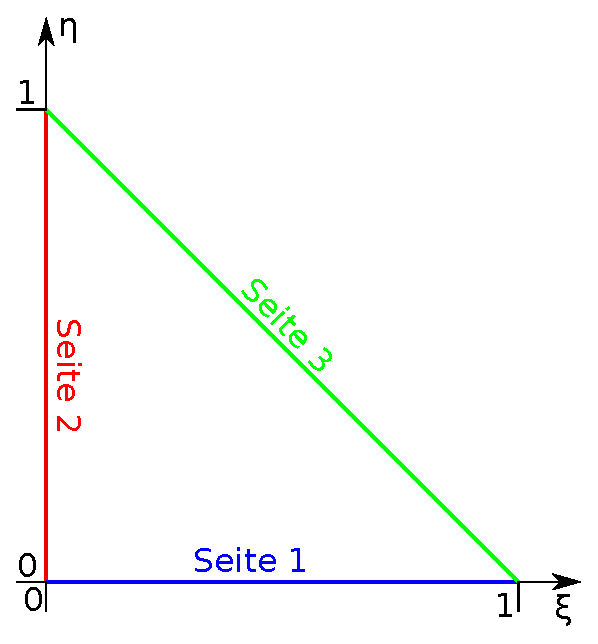
\includegraphics[scale=0.65]{pics/triangle_side_assignment.eps}
		\end{center}
		\caption{Zuordnung der Dreiecksseiten}
		\label{fig:triangle_side_assignment}
	\end{figure}
	\item Zu guter Letzt ordne man noch den Dreiecksseiten am Rand den Wert der Randbedingung (in (z.B. $\sigma$ aus \ref{eq:right_side_e_static}) ) zu.
\end{enumerate}

Um die in diesem Abschnitt gezeigten Zusammenhänge zu verdeutlichen, wird die Zuordnung der Dreiecksseiten zum neumannschen Rand anhand des in Abbildung \ref{fig:neumann_boundary_assignment} gezeigten Beispiels verdeutlicht. Eine Beispielhafte Gitterdatei ist in Code \ref{fig:example_mesh_file} gezeigt.

\lstinputlisting[frame=single, backgroundcolor=\color{lightgray}, basicstyle=\ttfamily\footnotesize, caption = {Exemplarische Gitterdatei}, label={fig:example_mesh_file}, captionpos=b ]{neumann_boundary_assignment_example_mesh_file.txt}

\begin{figure}[htbp]
	\begin{minipage}[t]{0.45\textwidth}
	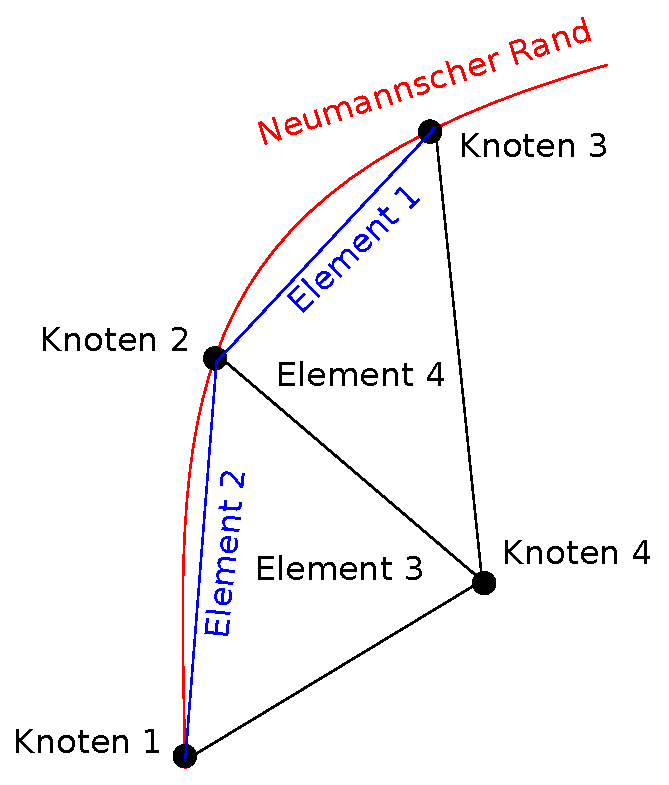
\includegraphics[scale=0.65]{pics/neumann_boundary_assignment.eps}
	\caption{Zuordnung der Dreiecksseiten}
	\label{fig:neumann_boundary_assignment}
	\end{minipage}
	\hfill
	\begin{minipage}[t]{0.45\textwidth}
	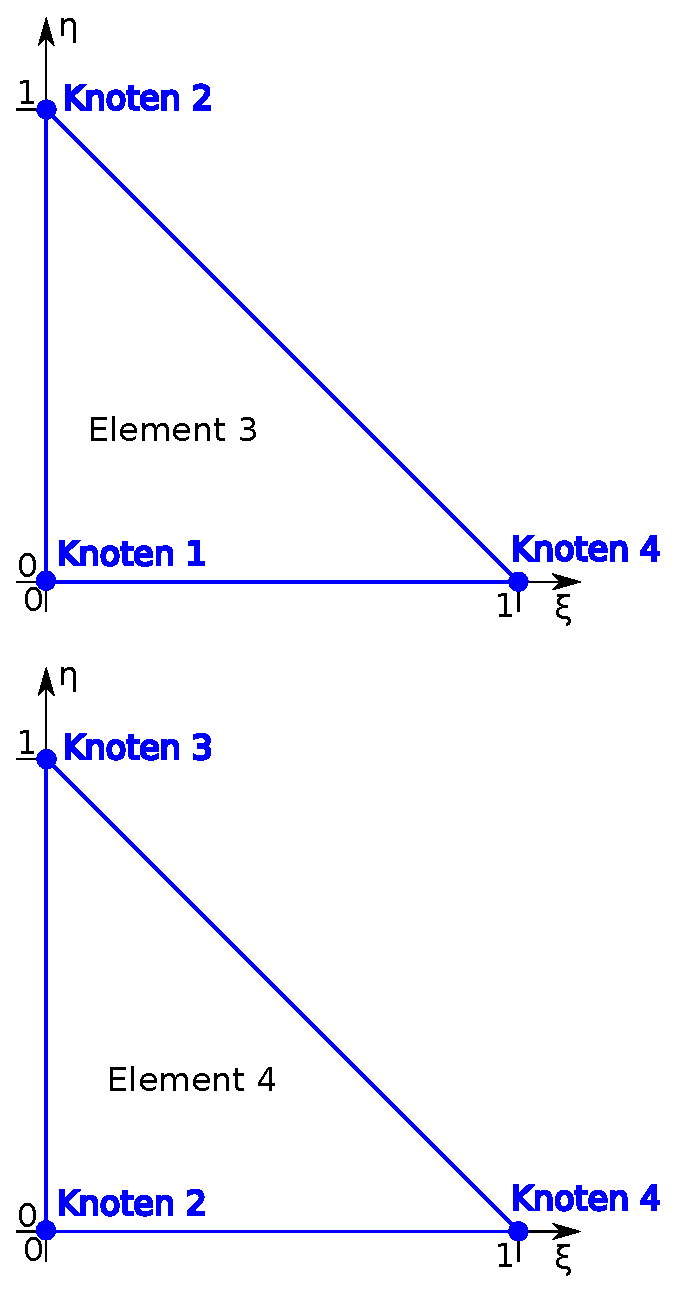
\includegraphics[scale=0.5]{pics/neumann_boundary_assignment_elements_3_4.eps}
	\caption{Elemente 3 und 4 im lokalen Koordinatensystem}
	\label{fig:neumann_boundary_assignment_elements_3_4}
	\end{minipage}	
\end{figure}	

Wie aus Code \ref{fig:example_mesh_file} ersichtlich, setzt sich die Geometrie aus 4 Knoten und 4 Elementen zusammen. Abbildung \ref{fig:neumann_boundary_assignment_elements_3_4} zeigt die Dreieckselemente 3 und 4 in ihrem lokalen Koordinatensystem. 

Wie mit Hilfe von Abbildung \ref{fig:triangle_side_assignment} zu erkennen ist, liegt Element 3 mit Seite 1, und Element 4 mit Seite 2 am neumannschen Rand. Der oben beschrieben Algorithmus wird nun auf dieses Beispiel angewandt um dessen Funktion zu erklären.\newline
\begin{enumerate}
	\item Die Elemente 1 und 2 sind, wie aus Code \ref{fig:example_mesh_file} ersichtlich der \textit{Physical grup} 1 zugeteilt. (Vierter Eintrag in den beiden Elementdefinitionen). Somit ist nun bekannt dass die Knoten 1, 2 und 3 am neumannschen Rand liegen.
	\item Die lokalen Knoten 1 und 2 von Element 3 stimmen mit den globalen Knoten 1 und 2 am neumannschen Rand überein, womit sich nun feststellen lässt dass Element 3 mit Seite 1 am neumannschen Rand liegt.
	\item Selbiges wir nun für Element 4 durchgeführt. Die lokalen Knoten 2 und 3 stimmen mit den globalen Knoten 2 und 3 überein, womit sich feststellen lässt dass Element 4 mit Seite 2 am neumannschen Rand liegt.
\end{enumerate}


\subsection{Berechnung der Elementgleichungssysteme}
\label{sec:equation_system_calculation}

Das Elementgleichungssystem in den Koordinaten $x$ und $y$ ergibt sich für ein elektrostatisches Problem als
\begin{equation}
\label{eq:k_ij_e_static_2}
k_{ij} = \int\displaylimits_{x} \int\displaylimits_{y} \left(\epsilon_x \parDiff{N_i}{x}\parDiff{N_j}{x} +  \epsilon_y\parDiff{N_i}{y}\parDiff{N_j}{y}\right)dx dy
\end{equation}

\begin{equation}
\label{eq:right_side_e_static_2}
r_j = \int\displaylimits_{x} \int\displaylimits_{y} N_i \rho dx dy + \int\displaylimits_{\Gamma_N} N_i\sigma d\Gamma
\end{equation} 
(siehe Kapitel \ref{sec:electrostatic_problems}). Die Berechnungen für stationäre Strömungsfeld-Probleme sind zu denen für elektrostatische Probleme äquivalent (Siehe Kapitel \ref{sec:stat_current_problems}) mit $\epsilon \rightarrow \gamma$, $\rho \rightarrow J_e$ und $\sigma \rightarrow 0$\newline

Liegt das Element am dirichletschen Rand, so sind ein oder mehrere Knotenpotentiale bereits vorgegeben was zu einer Reduktion des Elementgleichungssystems führt. Gezeigt wird dies an einem linearen Dreieckselement mit 3 Knoten. Das Elementgleichungssystem lautet:

\begin{align*}
	k_{11} V_1 + k_{12} V_2 + k_{13} V_3 = r_1\\
	k_{21} V_1 + k_{22} V_2 + k_{23} V_3 = r_2\\
	k_{31} V_1 + k_{32} V_2 + k_{33} V_3 = r_3
\end{align*}

Liegt nun Knoten 2 am dirichletschen Rand so ist $V_2$ bekannt, und das Elementgleichungssystem reduziert sich wie folgt:

 \begin{align*}
 k_{11} V_1  + k_{13} V_3 = r_1 - k_{12} V_2\\
 k_{31} V_1  + k_{33} V_3 = r_3 - k_{32} V_2
 \end{align*}
 
 Liegt also der $j$-te Knoten am dirichletschen Rand, so wird die $j$-te Zeile aus dem Gleichungssystem eliminiert und die $j$-ze Spalte wird von der rechte Seite subtrahiert.


\subsubsection{Elementmatrix-Koeffizienten $k_{ij}$}

Da die Formfunktionen $N_i$ bei isoparametrischen finiten Elementen Funktionen von $\xi$ und $\eta$ sind, müssen die Integrationsvariablen aller Integrale substituiert werden.  \newline
Die partiellen Ableitungen der Formfunktionen in (\ref{eq:k_ij_e_static_2}) ergeben nach \cite{SMS_VO_skript}, S.72 aus
\begin{equation}
\begin{Bmatrix}
\parDiff{N}{\xi} \\[2mm]
\parDiff{N}{\eta}
\end{Bmatrix} = 
\underbrace{
\begin{bmatrix}
\sum\limits_{k}\parDiff{N_k}{\xi}x_k & \sum\limits_{k}\parDiff{N_k}{\xi}y_k \\[2mm]
\sum\limits_{k}\parDiff{N_k}{\eta}x_k & \sum\limits_{k}\parDiff{N_k}{\eta}y_k
\end{bmatrix}}_{\mat{J}}\cdot
\begin{Bmatrix}
\parDiff{N}{x} \\[2mm]
\parDiff{N}{y}
\end{Bmatrix}
\end{equation}
zu
\begin{equation}
\label{eq:partial_derivatives_subst}
\begin{Bmatrix}
\parDiff{N}{x} \\[2mm]
\parDiff{N}{y}
\end{Bmatrix} = 
\underbrace{
	\frac{1}{\mathit{det}(\mat{J})}\begin{bmatrix}
	 \sum\limits_{k}\parDiff{N_k}{\eta}y_k & -\sum\limits_{k}\parDiff{N_k}{\xi}y_k \\[2mm]
	-\sum\limits_{k}\parDiff{N_k}{\eta}x_k & \sum\limits_{k}\parDiff{N_k}{\xi}x_k
	\end{bmatrix}}_{\mat{J}^{-1}}
\cdot \begin{Bmatrix}
\parDiff{N}{\xi} \\[2mm]
\parDiff{N}{\eta}
\end{Bmatrix}
\end{equation}


Das Flächenelement $dxdy$ in (\ref{eq:k_ij_e_static_2}) ergibt sich mit den Beziehungen aus \cite{SMS_VO_skript}, S.74 zu 
\begin{equation}
\label{eq:surface_element}
dxdy = \mathit{det} \mat{(J)} d\xi d\eta
\end{equation}
wobei das Flächenintegral in beiden Koordinaten in den Intervallen $\xi \in [0,1], \ \eta \in [0, 1-\xi]$ durchzuführen ist. Somit ergibt sich der Elementmatrix-Koeffizient $k_{ij}$ zu 
\begin{align}
&k_{i,j} = \int\displaylimits_{\xi = 0}^{1} \int\displaylimits_{\eta = 0}^{1 - \xi} \bigg[\\
%
% x-derivatives
&\frac{\epsilon_x}{\mathit{det}(\mat{J})}\left(\parDiff{N_i}{\xi}\sum\limits_{k}\parDiff{N_k}{\eta}y_k - \parDiff{N_i}{\eta}\sum\limits_{k}\parDiff{N_k}{\xi}y_k\right)
%
\left(\parDiff{N_j}{\xi}\sum\limits_{k}\parDiff{N_k}{\eta}y_k - \parDiff{N_j}{\eta} -\sum\limits_{k}\parDiff{N_k}{\xi}y_k\right) + \nonumber\\ 
%
% y-derivatives
&\frac{\epsilon_y}{\mathit{det}(\mat{J})}\left(-\parDiff{N_i}{\xi}\sum\limits_{k}\parDiff{N_k}{\eta}x_k + \parDiff{N_i}{\eta} \sum\limits_{k}\parDiff{N_k}{\xi}x_k\right)
%
\left(-\parDiff{N_j}{\xi}\sum\limits_{k}\parDiff{N_k}{\eta}x_k + \parDiff{N_j}{\eta} \sum\limits_{k}\parDiff{N_k}{\xi}x_k\right) \nonumber\\ 
& \bigg]d\xi d\eta
\end{align}

\textbf{Anmerkung:} Man beachte dass das $\mathit{det}(\mat{J})$ des Flächenelements aus (\ref{eq:surface_element}) bereits gekürzt wurde.\newline
Die Berechnung der Partiellen Ableitungen der Formfunktionen kann auf analytischem Wege vorweg erfolgen, da diese nur vom gewählten Elementtyp abhängen. Somit ist eine effiziente Berechnung der Terme $\sum\limits_{k}\parDiff{N_k}{\eta}y_k$ in Form von Skalarprodukten möglich.\newline

Die numerische Berechnung des Integrals erfolgt über die sogenannte \textit{Gauss-Quadratur}. Hierbei wird das zu berechnende Integral durch eine gewichtete Summe approximiert:
\begin{equation}
\int\limits_{x_{min}}^{x_{max}} f(x) dx \approx \sum\limits_{k}w_kf(x_k)
\end{equation}
Eine Erweiterung auf mehrdimensionale Integrale ist durch Mehrfachsummen einfach möglich. Ein besonderes Augenmerk bei dieser Methode der numerischen Integration liegt dabei auf der Wahl der Stützstellen $x_k$ und der Gewichte $w_k$. Die in dieser Arbeit verwendeten Stützstellen-Koordinaten und -Gewichte für isoparametrische Dreieckige finite Elemente wurden aus \cite{bathe}, S.547. übernommen. Implementiert sind eine 3-Punkte sowie eine 7-Punkte Integration.\newline

%In der Software implementiert sind eine 3-Punkte und 7-Punkte Integration der Form  
%\begin{equation}
%\int\displaylimits_{x} \int\displaylimits_{y} f dx dy \approx \frac{1}{2}\sum\limits_{k = 1}^{N_s} f(x_k, y_k) w_k
%\end{equation}
%wobei $N_s$ die Anzahl der Stützstellen darstellt.\newline
%
%Für eine 3-Punkte Integration ergeben sich folgende Stützstellen und Gewichte:
%\begin{table}[H]
%	\centering
%\begin{tabular}{c|c|c|c}
%	$\mathbf{k}$ & $\mathbf{x_k}$ & $\mathbf{y_k}$ & $\mathbf{w_k}$ \\
%	\hline
%	1 & $\frac{1}{6}$ & $\frac{1}{6}$ & $\frac{1}{3}$ \\
%	2 & $\frac{2}{3}$ & $\frac{1}{6}$ & $\frac{1}{3}$ \\
%	3 & $\frac{1}{6}$ & $\frac{2}{3}$ & $\frac{1}{3}$ \\
%\end{tabular}
%\caption{Stützstellen und Gewichte für 3-Punkte Integration nach \cite{bathe}, S.547.}
%\label{tab:3-point_plane_integration}
%\end{table}
%
%Für eine 7-Punkte Integration ergeben sich folgende Stützstellen und Gewichte:
%\begin{table}[H]
%	\centering
%	\begin{tabular}{c|c|c|c}
%		$\mathbf{k}$ & $\mathbf{x_k}$ & $\mathbf{y_k}$ & $\mathbf{w_k}$ \\
%		\hline
%		1 & $0.1012865073235$ & $0.1012865073235$ & $0.1259391805448$ \\
%		2 & $0.7974269853531$ & $0.1012865073235$ & $0.1259391805448$ \\
%		3 & $0.1012865073235$ & $0.7974269853531$ & $0.1259391805448$ \\
%		4 & $0.4701420641051$ & $0.0597158717898$ & $0.1323941527885$ \\
%		5 & $0.4701420641051$ & $0.4701420641051$ & $0.1323941527885$ \\
%		6 & $0.0597158717898$ & $0.4701420641051$ & $0.1323941527885$ \\
%		7 & $\frac{1}{3}$ & $\frac{1}{3}$ & $0.225$ \\
%	\end{tabular}
%	\caption{Stützstellen und Gewichte für 7-Punkte Integration nach \cite{bathe}, S.547.}
%	\label{tab:7-point_plane_integration}
%\end{table}



\subsubsection{Rechtsseiten-Elemente $r_j$}
Die Berechnung der Koeffizienten der 'rechten Seite' eines elektrostatischen Problems 
\begin{equation}
r_j = \int\displaylimits_{x} \int\displaylimits_{y} N_i \rho dx dy + \int\displaylimits_{\Gamma_N} N_i\sigma d\Gamma
\end{equation}$r_j$
erfordert zu einen ein Flächenintegral (erster Summand) und ein Integral über den neumannschen Rand, welches im zweidimensionalen Fall zu einem Kurvenintegral entartet. \newline
Für das Flächenintegral lässt sich die Substitution der Integrationsvariablen sehr einfach durchführen, da keine partiellen Ableitungen des Formfunktionen vorkommen:
\begin{equation}
\int\displaylimits_{x} \int\displaylimits_{y} N_i \rho dx dy = \int\displaylimits_{\xi = 0}^{1} \int\displaylimits_{\eta = 0}^{1 - \xi} N_i \rho \mathit{det} (\mat{J}) d\xi d\eta
\end{equation}
\newline

Für Kurvenintegral über den neumannschen Rand ändert sich der Integrand je nach dem über welche Dreiecksseite integriert wird. 
Das entartete Flächenintegral über den neumannschen Rand hat nun folgende Form:
\begin{equation}
	\int\displaylimits_{c}N_i(\xi, \eta)\sigma ds
\end{equation}

Allgemein gilt (siehe \cite{SMS_VO_skript}, S. 74f.):
\begin{align}
\label{eq:subs}
\vec{d\xi} = dx\vec{e_x} + dy\vec{e_y} = \parDiff{x}{\xi}d\xi \vec{e_x} + \parDiff{x}{\xi} d\xi \vec{e_y}\\
\vec{d\eta} = dx\vec{e_x} + dy\vec{e_y} = \parDiff{x}{\eta}d\eta \vec{e_x} + \parDiff{x}{\eta} d\eta \vec{e_y} \nonumber
\end{align}
Das infinitesimale Kurvenelement ergibt sich somit nun zu $\vec{ds} = \vec{d\xi} + \vec{d\eta}$ bzw. \begin{equation}
\label{eq:ds_abs}
ds = \left|\left| \vec{ds} \right|\right| = \sqrt{\left(\vec{d\xi} + \vec{d\eta}\right)^T\cdot \left( \vec{d\xi} + \vec{d\eta} \right)}
\end{equation}\newline

Integriert man über die Dreiecksseite 1, so gilt $d\eta = 0$ und somit auch $\vec{d\eta} = \vec{0}$.
Somit gilt für $\vec{ds}$ bzw. $ds$:
\begin{align}
	&\vec{ds} =  \vec{d\xi} \Rightarrow \nonumber \\
	&ds = \left|\left| \vec{d\xi} \right|\right| = \sqrt{ \left(\parDiff{x}{\xi}\right)^2 + \left(\parDiff{y}{\xi}\right)^2) d\xi} = \sqrt{ \left( \sum\limits_{k}\parDiff{N_k}{\xi}x_k \right)^2  + \left( \sum\limits_{k}\parDiff{N_k}{\xi}y_k \right)^2 } d\xi
\end{align}

Selbiges kann für Dreiecksseite 2 unter Verwendung von $d\xi = 0$ hergeleitet werden. Es ergibt sich somit:
\begin{align}
&\vec{ds} =  \vec{d\eta} \Rightarrow \nonumber \\
&ds = \left|\left| \vec{d\eta} \right|\right| = \sqrt{ \left(\parDiff{x}{\eta}\right)^2 + \left(\parDiff{y}{\eta}\right)^2) d\eta} = \sqrt{ \left( \sum\limits_{k}\parDiff{N_k}{\eta}x_k \right)^2  + \left( \sum\limits_{k}\parDiff{N_k}{\eta}y_k \right)^2 } d\eta
\end{align}

Zur Integration über Dreiecksseite 3  muss zuerst die Kurve parametrisiert werden:
\begin{align*}
&\vec{s(t)} = 
\begin{Bmatrix}
\xi(t) \\ \eta(t)
\end{Bmatrix} = 
\begin{Bmatrix}
1 - t \\ t
\end{Bmatrix} \Rightarrow\\
%
&\frac{ds}{dt} = 
\begin{Bmatrix}
\frac{d\xi}{dt} \\ \frac{d\eta}{dt}
\end{Bmatrix} = 
\begin{Bmatrix}
-1 \\ 1
\end{Bmatrix} \Rightarrow \\
% 
&\underline{\underline{d\xi = -dt, \ d\eta = dt}}
\end{align*}

Setzt man dies nun in (\ref{eq:subs}) und dies wiederum in (\ref{eq:ds_abs}) ein, so erhält man
\begin{equation}
ds = \sqrt{\left(\parDiff{x}{\eta} - \parDiff{x}{\xi}\right)^2  + \left(\parDiff{y}{\eta} - \parDiff{y}{\xi}\right)^2} dt
\end{equation}

Auf das Einsetzen der partiellen Ableitungen von $x$ und $y$ wurde aus Gründen der Übersichtlichkeit verzichtet.\newline


Die numerische Integration erfolgt wieder über die Gauss-Quadratur. Stützstellen und Gewichte wurden aus \cite{bathe}, S.542 übernommen.


\subsection{Assemblierung und Lösung des globalen Gleichungssystems}
\label{sec:assembling}
Im vorherigen Abschnitt wurde näher auf die Berechnung der Elementgleichungssysteme eingegangen. Diese müssen nun zu einem 'großen' Gleichungssystem assembliert werden. Der Assemblierungsvorgang entspricht dabei einer simplen Addition der Gleichungssysteme (Siehe \cite{SMS_VO_Skript}, S.60ff.). Beispielhaft wird der Vorgang anhand von 2 Elementgleichungssystemen gezeigt.

Gleichungssystem 1:
\begin{align*}
k_{11}^1 V_1 + k_{12}^1 V_2 + k_{13}^1 V_3 = r_1^1\\
k_{21}^1 V_1 + k_{22}^1 V_2 + k_{23}^1 V_3 = r_2^1\\
k_{31}^1 V_1 + k_{32}^1 V_2 + k_{33}^1 V_3 = r_3^1
\end{align*}


Gleichungssystem 2:
\begin{align*}
k_{22}^2 V_2 + k_{23}^2 V_3 = r_2^2 - k_{21}^2 V_4\\
k_{32}^2 V_2 + k_{33}^2 V_3 = r_3^2 - k_{31}^2 V_4
\end{align*}

Addiert man die Gleichungssysteme so ergibt sich
\begin{align}
k_{11}^1 V_1 + k_{12}^1 V_2 + k_{13}^1 V_3 +  &= r_1^1\\
k_{21}^1 V_1 + (k_{22}^1 +  k_{22}^2) V_2 + (k_{23}^1 + k_{23}^2) V_3 &= r_2^1 + r_2^2 - k_{21}^2 V_4 \nonumber\\
k_{31}^1 V_1 + (k_{32}^1 + k_{32}^2)  V_2 + ( k_{33}^1 + k_{33}^2) V_3 &= r_3^1 + r_3^2 - k_{31}^2 V_4 \nonumber
\end{align}

Als Resultat des Assemblierungsvorgangs erhält man ein lineares Gleichungssystem mit $N - N_{dir}$ Unbekannten, wobei $N$ die Anzahl der Knoten und $N_{dir}$ die Anzahl der Knoten am dirichletschen Rand darstellt. Die Koeffizientenmatrix ist symmetrisch und schwach besetzt.
\newline

Die Lösung des Gleichungssystems erfolgt durch ein geeignetes Verfahren und liefert die Unbekannten Knotenpotentiale als Ergebnis. Je nach zugrundeliegendem Problemtyp kann anschließend die gesuchter Feldgröße berechnet werden. Für den Fall eines elektrostatischen Problems wäre dies
\begin{equation}
\vec{E} = -\mathit{grad}V = 
-\begin{Bmatrix}
\parDiff{V}{x} \\[2mm]
\parDiff{V}{y}
\end{Bmatrix} = 
%
-\begin{Bmatrix}
\sum_{k} \parDiff{N_k}{x} V_k\\[2mm]
\sum_{k} \parDiff{N_k}{y} V_k
\end{Bmatrix}
\end{equation}
mit 
\begin{align*}
\parDiff{N_k}{x} = \frac{1}{\mathit{det}(\mat{J})} \left( \parDiff{N_k}{\xi} \sum_{j} \parDiff{N_j}{\eta} y_j - \parDiff{N_k}{\eta} \sum_{j} \parDiff{N_j}{\xi} y_j \right) \\
\parDiff{N_k}{y} = \frac{1}{\mathit{det}(\mat{J})} \left( -\parDiff{N_k}{\xi} \sum_{j} \parDiff{N_j}{\eta} x_j + \parDiff{N_k}{\eta} \sum_{j} \parDiff{N_j}{\xi} x_j \right) \\
\end{align*}



\newpage
\section{Simulationen}
Sofern nicht anders angegeben werden 6-knotige quadratische finite Dreieckselemente zur Approximation der Geometrie verwendet.

\subsection{Beispiel 1: Idealer Plattenkondensator}
In diesem Beispiel wird ein idealer Plattenkondensator unter Vernachlässigung der Randeffekte berechnet. Für ein solches Problem existiert eine analytische Lösung mit einem linearen Potentialverlauf und einem konstanten elektrischen Feld $\vec{E} = \frac{U}{d}$ mit $d$ als Plattenabstand.\newline

Für dieses Problem liefert der FEM-Algorithmus die exakte Lösung liefern, da ein quadratischer Approximationsansatz verwendet wird und der Potentialverlauf ein Linearer ist.



Folgende Parameter sind gegeben: 
\begin{itemize}
	\item $U = 10 \si{\volt}$
	\item $d = 1 \si{\milli\meter}$
	\item $\epsilon = \epsilon_0$
\end{itemize}

woraus sich ein Potentialverlauf von $V(x) = 10000x$ mit $x = [0,d]$ und ein Elektrischen Feld von $E = 10000 \si{\volt\per\meter}$ ergibt.

\begin{figure}[htbp]
	\centering
	\includegraphics[width=\textwidth]{pics/example_1/geometry.eps}
	\caption{Geometrie, Gitter und Randbedingungen zu Beispiel 1}
\end{figure}
\textbf{Anmerkung:} Die homogenen neumannschen Randbedingungen $\parDiff{V}{n} = 0$ müssen nicht explizit angegeben werden.


\begin{figure}[htbp]
	\begin{minipage}{0.5\textwidth}
		\includegraphics[width=\textwidth]{pics/example_1/figure_4.eps}
	\end{minipage}
	\begin{minipage}{0.5\textwidth}
		\includegraphics[width=\textwidth]{pics/example_1/figure_3.eps}
	\end{minipage}
\caption{Potentialverlauf des Plattenkondensators}
\label{fig:plate_cape_potential}
\end{figure}

\begin{figure}[htbp]
	\begin{minipage}{0.5\textwidth}
		\includegraphics[width=\textwidth]{pics/example_1/figure_5.eps}
	\end{minipage}
	\begin{minipage}{0.5\textwidth}
		\includegraphics[width=\textwidth]{pics/example_1/figure_6.eps}
	\end{minipage}
	\caption{Feldverlauf des Plattenkondensators}
	\label{fig:plate_cape_field}
\end{figure}

Abbildung \ref{fig:plate_cape_potential} zeigt den linearen Potentialverlauf innerhalb des Kondensators. Abbildung \ref{fig:plate_cape_field} zeigt im linken Teil die (nicht skalierten) Feldlinien und im rechten Teil den Absolutwert des Feldes.


\subsection{Beispiel 2: Strömungsfeld einer Blechplatte}
Dieses Beispiel zeigt den Strömungsfeldverlauf einer Blechplatte und wurde aus \cite{SMS_VO_skript}, Kap. 7.2.1 übernommen.\newline

\begin{figure}[H]
	\centering
	\includegraphics[scale=0.28]{pics/example_2/geometry.eps}
	\caption{Geometrie, Gitter und Randbedingungen zu Beispiel 2}
\end{figure}

Abbildung \ref{fig:metal_plate_potential} zeigt wieder den Verlauf des berechneten Potentials. Im linken Teil der Abbildung ist zu beachten dass der Potentialverlauf innerhalb des inneren, rechteckigen Randes zu ignorieren ist. Er wurde lediglich durch den Algorithmus zur Generierung des Bildes hinzugefügt und besitzt somit keinerlei physikalische Bedeutung.\newline

\begin{figure}[htbp]
	\begin{minipage}{0.5\textwidth}
		\includegraphics[width=\textwidth]{pics/example_2/figure_4.eps}
	\end{minipage}
	\begin{minipage}{0.5\textwidth}
		\includegraphics[width=\textwidth]{pics/example_2/figure_3.eps}
	\end{minipage}
	\caption{Potentialverlauf der Blechplatte}
	\label{fig:metal_plate_potential}
\end{figure}


Abbildung \ref{fig:metal_plate_field} zeigt den Feldverlauf des Strömungsfeldes. Das Strömungsfeld wurde über $\vec{J} = -[\gamma] \mathit{grad}V$ berechnet, wobei $[\gamma] = \begin{bmatrix}1 & 0 \\ 0 & 1\end{bmatrix}$ gewählt wurde. Somit entspricht bei diesem Beispiel $\vec{J} = \vec{E}$.\newline
Wie zu erwarten tritt an der Ecke des inneren Randes eine starke Konzentration des Feldes mit einem entsprechend hohen Absolutwert des Feldes auf. Bei der Generierung des Gitters ist hier auf eine entsprechende Auflösung zu achten.
\begin{figure}[htbp]
	\begin{minipage}{0.5\textwidth}
		\includegraphics[width=\textwidth]{pics/example_2/figure_5.eps}
	\end{minipage}
	\begin{minipage}{0.5\textwidth}
		\includegraphics[width=\textwidth]{pics/example_2/figure_6.eps}
	\end{minipage}
	\caption{Feldverlauf der Blechplatte}
	\label{fig:metal_plate_field}
\end{figure}


\subsection{Beispiel 3: Zylinderelektroden über leitender Ebene}
Dieses Beispiel zeigt den Feldverlauf zweier Zylinderelektroden über einer leitenden Ebene. Die Elektroden befinden sich $100 \si{\milli\meter}$ bzw. $200 \si{\milli\meter}$ in einem Abstand von $100 \si{\milli\meter}$ über der leitenden Ebene. Die Ebene besitzt ein Potential von $V = 0 \si{\volt}$

\begin{figure}[H]
	\begin{minipage}{0.5\textwidth}
		\includegraphics[width=\textwidth]{pics/example_3/geometry_full.eps}
	\end{minipage}
	\begin{minipage}{0.5\textwidth}
		\includegraphics[width=\textwidth]{pics/example_3/geometry.eps}
	\end{minipage}
	\caption{Geometrie, Gitter und Randbedingungen zu Beispiel 3}
	\label{fig:example_3_geometry}
\end{figure}

Abbildung \ref{fig:example_3_geometry} zeigt die Geometrie sowie das Gitter und die Randbedingungen des Problems. Im linken Teil erkennt man die gesamte Geometrie inklusive fernem Rand. Im rechten Teil ist der interessante Teil der Geometrie mit den Zylinderelektroden dargestellt. 

\begin{figure}[htbp]
	\begin{minipage}{0.5\textwidth}
		\includegraphics[width=\textwidth]{pics/example_3/figure_4.eps}
	\end{minipage}
	\begin{minipage}{0.5\textwidth}
		\includegraphics[width=\textwidth]{pics/example_3/figure_3_edited.eps}
	\end{minipage}
	\caption{Potentialverlauf der Zylinderelektroden}
	\label{fig:cylinder_electrodes_potential}
\end{figure}

Abbildung \ref{fig:cylinder_electrodes_potential} zeigt wie bereits bekannt den Potentialverlauf des Problems. Hier ist zu beachten dass beim rechten Teil die Ansicht um 180\degrees gedreht ist, was im linken Teil einer Blickrichtung von oben nach unten entspricht. Diese Ansicht wurde gewählt da sich sonst die Äquipotentialfläche der ersten Elektrode nur schwer zu erkennen ist.


\begin{figure}[htbp]
	\begin{minipage}{0.5\textwidth}
		\includegraphics[width=\textwidth]{pics/example_3/figure_5.eps}
	\end{minipage}
	\begin{minipage}{0.5\textwidth}
		\includegraphics[width=\textwidth]{pics/example_3/figure_6.eps}
	\end{minipage}
	\caption{Feldverlauf der Zylinderelektroden}
	\label{fig:cylinder_electrodes_field}
\end{figure}


Abbildung \ref{fig:cylinder_electrodes_field} zeigt den Feldverlauf und den Absolutwert des Elektrischen Feldes.

\appendix
\section{Formfunktionen und ihre partiellen Ableitungen}
\label{sec:annex_shape_functions}
\subsection{Lineare Dreieckselemente}
\label{sec:linear_triangles_annex}

\begin{minipage}[t]{0.3\textwidth}
\subsubsection{Formfunktionen}
\begin{align*}
	&N_1 = 1 - \xi - \eta\\
	&N_2 = \xi \\
	&N_3 = \eta
\end{align*}
\end{minipage}
\begin{minipage}[t]{0.3\textwidth}
\subsubsection{Partielle Ableitungen nach $\xi$}
\begin{align*}
&\parDiff{N1}{\xi} = -1\\
&\parDiff{N_2}{\xi} = 1\\
&\parDiff{N_3}{\xi} = 0
\end{align*}
\end{minipage}
\begin{minipage}[t]{0.3\textwidth}
\subsubsection{Partielle Ableitungen nach $\eta$}
\begin{align*}
&\parDiff{N_1}{\eta} = -1\\
&\parDiff{N_2}{\eta} = 0\\
&\parDiff{N_3}{\eta} = 1
\end{align*}
\end{minipage}



\subsection{Quadratische Dreieckselemente}
\label{sec:quadratic_triangles_annex}
\begin{minipage}[t]{0.3\textwidth}
\subsubsection{Formfunktionen}
\begin{align*}
&N_1 = (1 - \xi - \eta)(1 - 2\xi - 2\eta)\\
&N_2 = 4\xi (1 - \xi - \eta) \\
&N_3 = \xi (2 \xi - 1)\\
&N_4 = 4 \xi \eta \\
&N_5 = \eta (2\eta - 1)\\
&N_6 = -4\eta (1 - \xi - \eta)
\end{align*}
\end{minipage}
\begin{minipage}[t]{0.3\textwidth}
\subsubsection{Partielle Ableitungen nach $\xi$}
\begin{align*}
&\parDiff{N_1}{\xi} = -3 + 4\xi + 4\eta\\
&\parDiff{N_2}{\xi} = 4 - 8\xi - 4\eta\\
&\parDiff{N_3}{\xi} = 4\xi - 1\\
&\parDiff{N_4}{\xi} = 4\eta\\
&\parDiff{N_5}{\xi} = 0\\
&\parDiff{N_6}{\xi} = -4\eta\\
\end{align*}
\end{minipage}
\begin{minipage}[t]{0.3\textwidth}
\subsubsection{Partielle Ableitungen nach $\eta$}
\begin{align*}
&\parDiff{N_1}{\eta} = -3 + 4\xi + 4\eta\\
&\parDiff{N_2}{\eta} = -4\xi \\
&\parDiff{N_3}{\eta} = 0\\
&\parDiff{N_4}{\eta} = 4\xi\\
&\parDiff{N_5}{\eta} = 4\eta - 1\\
&\parDiff{N_6}{\eta} = 4 - 4\xi - 8\eta\\
\end{align*}
\end{minipage}

\subsection{Kubische Dreieckselemente}
\label{sec:cubic_triangles_annex}
\subsubsection{Formfunktionen}

\begin{align*}
&N_1 = -\frac{9\eta ^3}{2}-\frac{27\eta ^2\xi}{2}+9\eta ^2-\frac{27\eta {\xi}^2}{2}+18\eta \xi-\frac{11\eta }{2}-\frac{9{\xi}^3}{2}+9{\xi}^2-\frac{11\xi}{2}+1\\
&N_2 = \frac{27\eta ^2\xi}{2}+27\eta {\xi}^2-\frac{45\eta \xi}{2}+\frac{27{\xi}^3}{2}-\frac{45{\xi}^2}{2}+9\xi \\
&N_3 = \frac{9\eta \xi}{2}-\frac{9\xi}{2}-\frac{27\eta {\xi}^2}{2}+18{\xi}^2-\frac{27{\xi}^3}{2}\\
&N_4 = \frac{9{\xi}^3}{2}-\frac{9{\xi}^2}{2}+\xi \\
&N_5 = \frac{27\eta {\xi}^2}{2}-\frac{9\eta \xi}{2}\\
&N_6 = \frac{27\eta ^2\xi}{2}-\frac{9\eta \xi}{2}\\
&N_7 = \frac{9\eta ^3}{2}-\frac{9\eta ^2}{2}+\eta \\
&N_8 = \frac{9\eta \xi}{2}-\frac{9\eta }{2}-\frac{27\eta ^2\xi}{2}+18\eta ^2-\frac{27\eta ^3}{2}\\
&N_9 = \frac{27\eta ^3}{2}+27\eta ^2\xi-\frac{45\eta ^2}{2}+\frac{27\eta {\xi}^2}{2}-\frac{45\eta \xi}{2}+9\eta \\
&N_{10} = -27\eta ^2\xi-27\eta {\xi}^2+27\eta \xi
\end{align*}

\begin{minipage}[t]{0.45\textwidth}

\subsubsection{Partielle Ableitungen nach $\xi$}
\begin{align*}
&\parDiff{N_1}{\xi} = -\frac{27\eta ^2}{2}-27\eta \zeta+18\eta -\frac{27{\zeta}^2}{2}+18\zeta-\frac{11}{2}\\
&\parDiff{N_2}{\xi} = \frac{27\eta ^2}{2}+54\eta \zeta-\frac{45\eta }{2}+\frac{81{\zeta}^2}{2}-45\zeta+9\\
&\parDiff{N_3}{\xi} = \frac{9\eta }{2}+36\zeta-27\eta \zeta-\frac{81{\zeta}^2}{2}-\frac{9}{2}\\
&\parDiff{N_4}{\xi} = \frac{27{\zeta}^2}{2}-9\zeta+1\\
&\parDiff{N_5}{\xi} = 27\eta \zeta-\frac{9\eta }{2}\\
&\parDiff{N_6}{\xi} = \frac{27\eta ^2}{2}-\frac{9\eta }{2}\\
&\parDiff{N_7}{\xi} = 0\\
&\parDiff{N_8}{\xi} = \frac{9\eta }{2}-\frac{27\eta ^2}{2}\\
&\parDiff{N_9}{\xi} = 27\eta \zeta-\frac{45\eta }{2}+27\eta ^2\\
&\parDiff{N_{10}}{\xi} = 27\eta -54\eta \zeta-27\eta ^2\\
\end{align*}
\end{minipage}
\hspace{5mm}
\begin{minipage}[t]{0.45\textwidth}
\subsubsection{Partielle Ableitungen nach $\eta$}
\begin{align*}
&\parDiff{N_1}{\eta} = -\frac{27\eta ^2}{2}-27\eta \zeta+18\eta -\frac{27{\zeta}^2}{2}+18\zeta-\frac{11}{2}\\
&\parDiff{N_2}{\eta} = 27\eta \zeta-\frac{45\zeta}{2}+27{\zeta}^2\\
&\parDiff{N_3}{\eta} = \frac{9\zeta}{2}-\frac{27{\zeta}^2}{2}\\
&\parDiff{N_4}{\eta} = 0\\
&\parDiff{N_5}{\eta} = \frac{27{\zeta}^2}{2}-\frac{9\zeta}{2}\\
&\parDiff{N_6}{\eta} = 27\eta \zeta-\frac{9\zeta}{2}\\
&\parDiff{N_7}{\eta} = \frac{27\eta ^2}{2}-9\eta +1\\
&\parDiff{N_8}{\eta} = 36\eta +\frac{9\zeta}{2}-27\eta \zeta-\frac{81\eta ^2}{2}-\frac{9}{2}\\
&\parDiff{N_9}{\eta} = \frac{81\eta ^2}{2}+54\eta \zeta-45\eta +\frac{27{\zeta}^2}{2}-\frac{45\zeta}{2}+9\\
&\parDiff{N_{10}}{\eta} = 27\zeta-54\eta \zeta-27{\zeta}^2\\
\end{align*}
\end{minipage}




\newpage
\addcontentsline{toc}{section}{Literatur}
\bibliography{literatur}

\end{document}